%% Artigo TCC -- iCEV, Engenharia de Software.
%% Formatacao conforme "Manual do TCC" (iCEV, Setembro/2025), Anexo I:
%% Times New Roman 12, espacamento 1,5, texto justificado, recuo de paragrafo
%% 1,25cm, margens superior e esquerda 3cm, inferior e direita 2cm.
%% Esta versao NAO e cega: identifica autor, orientador e a instituicao estudada.
\documentclass[12pt,a4paper]{article}

\usepackage[T1]{fontenc}
\usepackage[utf8]{inputenc}
\usepackage[brazilian]{babel}
\usepackage{newtxtext,newtxmath}
\usepackage[top=3cm,left=3cm,bottom=2cm,right=2cm]{geometry}
\usepackage{setspace}
\usepackage{indentfirst}
\usepackage{booktabs}
\usepackage{longtable}
\usepackage{array}
\usepackage{graphicx}
\graphicspath{{figures/}{../figures/}}
\usepackage{amsmath}
\usepackage{ragged2e}
\usepackage{footmisc}
\usepackage{xurl}
\usepackage{pdfpages}
\usepackage[hidelinks]{hyperref}
\usepackage[alf]{abntex2cite}

\setlength{\parindent}{1.25cm}
\setlength{\parskip}{0pt}
\setlength{\emergencystretch}{3em}

%% Citacao longa: mais de 3 linhas -> fonte 10, recuo 4cm, espacamento simples.
\newenvironment{citacao}
  {\begin{list}{}{\setlength{\leftmargin}{4cm}\setlength{\rightmargin}{0pt}}%
   \item[]\begin{singlespace}\fontsize{10}{12}\selectfont}
  {\end{singlespace}\end{list}}

%% Titulos de secao em corpo 12, sem numeracao automatica -- o Anexo I usa
%% "Introducao", "Capitulo de Desenvolvimento", "Consideracoes Finais".
\usepackage{titlesec}
\titleformat{\section}{\normalsize\bfseries}{\thesection}{0.5em}{}
\titleformat{\subsection}{\normalsize\bfseries\itshape}{\thesubsection}{0.5em}{}
\titleformat{\subsubsection}{\normalsize\itshape}{\thesubsubsection}{0.5em}{}
\titlespacing*{\section}{0pt}{1.5\baselineskip}{0.5\baselineskip}
\titlespacing*{\subsection}{0pt}{1.2\baselineskip}{0.4\baselineskip}
\titlespacing*{\subsubsection}{0pt}{1.0\baselineskip}{0.3\baselineskip}

\newcommand{\TITULO}{Modelagem de tipos de processo administrativo e de caminhos típicos
a partir de registros de atividades}
\newcommand{\SUBTITULO}{um catálogo auditável para a transparência e otimização administrativa}
\newcommand{\AUTOR}{Gabriel Feitosa Melo Coelho}
\newcommand{\ORIENTADOR}{Prof. Dr. Dimmy Karson Soares Magalhães}

\begin{document}
\onehalfspacing
\justifying

\begin{center}
{\bfseries\large \TITULO}\\[2pt]
{\large \SUBTITULO}
\end{center}

\vspace{1.5\baselineskip}

\begin{flushright}
\AUTOR\footnote{Graduando em Engenharia de Software pelo Instituto de Ensino Superior
iCEV. E-mail: gabrielcoelho09gc@gmail.com.}\\
\ORIENTADOR\footnote{Orientador. Doutor. Docente do curso de Engenharia de Software do
Instituto de Ensino Superior iCEV. Email: }
\end{flushright}

\vspace{1.5\baselineskip}

\noindent\textbf{Resumo:}

\noindent Embora a legislação de transparência exija o mapeamento de procedimentos administrativos, sistemas como o Sistema Eletrônico de Informações (SEI) registram ações isoladas sem consolidar o fluxo real dos processos. O problema desta pesquisa consiste em determinar se é possível extrair, a partir de registros transacionais brutos, um catálogo auditável e confiável dos procedimentos efetivamente executados. Trata-se de uma pesquisa aplicada e quantitativa, conduzida como estudo de caso na Secretaria de Administração do Estado do Piauí (SEAD-PI), analisando 5.243 processos concluídos em 2025. Propõe-se um \emph{pipeline} que modela os eventos como um grafo de conhecimento e agrupa os processos combinando o texto do documento inicial ao histórico de tramitação. Para predizer o caminho típico de cada processo, avaliaram-se seis famílias de modelos (incluindo cadeias de Markov e arquiteturas GRU), testadas em três alfabetos de traço: ação por unidade, roteamento e procedimento. Os resultados mostram ganhos preditivos consistentes contra partições-controle embaralhadas em todas as 252 comparações. Comparado a um modelo global, obteve-se ganho preditivo significativo apenas no alfabeto de procedimento (0,109 com Markov de terceira ordem e 0,131 com GRU). As métricas internas de clusterização não apontaram um agrupamento único ideal. Contudo, a aplicação das técnicas gerou um catálogo validado de 60 tipos de processos, com 75,1\% de cobertura no alfabeto de roteamento, atendendo aos requisitos estritos de anonimização. Conclui-se que o uso de inteligência artificial sobre \emph{logs} administrativos supre a lacuna empírica dos sistemas, viabilizando a governança orientada a dados.

\vspace{0.6\baselineskip}
\noindent\textbf{Palavras-chave:} \textit{mineração de processos; inteligência artificial; redes neurais; otimização; transparência administrativa}.

\vspace{1.2\baselineskip}
\noindent\textbf{Abstract:}

\noindent Access-to-information laws presume the existence of consolidated records for administrative procedures, which often are never created. This research investigates whether an auditable catalogue of executed process types and their typical paths can be derived directly from raw event logs. We conducted an applied, quantitative single-case study at the Secretariat of Administration of the State of Piaui, analyzing 5,243 concluded cases from the Electronic Information System (SEI) in 2025. The methodology builds an event knowledge graph, clusters cases by combining opening-document text with routing and action history, and fits typical paths using six model families across three trace alphabets (action-by-unit, routing, and procedure). Results show positive predictive gains over shuffled control partitions in all 252 baseline comparisons. Compared to a single global model, predictive gains were significant only in the procedure alphabet (0.109 for a third-order Markov chain; 0.131 for GRU); in action-by-unit and routing, gains were indistinguishable from residuals. Although accuracy separated the 14 candidate clusterings by only 0.0055 and internal indices did not reliably predict downstream quality, the pipeline successfully delivered a catalogue of 60 process types with 0.751 coverage in the routing alphabet. Furthermore, the required automated anonymization proved non-inferior at the pre-registered margin across all 54 comparisons.

\vspace{0.6\baselineskip}
\noindent\textbf{Keywords:} \textit{process mining; clustering; graphs; administrative transparency}.

\newpage

\section{INTRODUÇÃO}

O direito de acesso à informação pressupõe que a administração pública conheça os seus próprios fluxos de trabalho. Regimes de transparência ativa e mandatos de dados abertos frequentemente operam sob a premissa de que os relatos da prática administrativa já existem e aguardam apenas publicação. Contudo, \citeonline{brauneis2018algorithmic} testaram esse pressuposto empiricamente e constataram que o maior obstáculo à transparência não é o sigilo, mas a inexistência prévia desses registros consolidados.

Os sistemas eletrônicos de processo administrativo mitigam parcialmente esse problema. O Sistema Eletrônico de Informações (SEI), por exemplo, registra eventos atômicos para cada processo, como a unidade recebedora e a ação executada. Embora o rastro transacional exista, falta a consolidação que traduza esses dados agregados em conhecimento útil sobre quais procedimentos a administração de fato executa e como tramitam. As administrações mantêm uma taxonomia oficial de tipos de processo, mas esta é aplicada manualmente no momento da abertura do caso. Consequentemente, a sua precisão em relação à prática efetiva é uma questão empírica. 

Há uma limitação técnica no SEI que inviabiliza presumir a validade dessa taxonomia: o sistema não impõe restrições de sequência de atividades por tipo de processo. Dois casos de um mesmo tipo declarado podem seguir fluxos inteiramente distintos. Por essa razão, a taxonomia oficial entra neste trabalho como uma hipótese a ser testada, exigindo que o catálogo de processos seja derivado diretamente dos registros transacionais (Seção 2.2.7).

No ordenamento brasileiro, a relevância dessa derivação é acentuada pelo dever legal de publicar as principais etapas de cada procedimento em formato legível por máquina. A discussão sobre o alcance material desse dever sobre o corpus estudado é aprofundada na Seção 2.2.5.

A motivação desta pesquisa advém de um contexto prático. Atuo como analista de dados da Secretaria de Administração do Estado do Piauí (SEAD-PI) e sou graduando em Engenharia de Software pelo iCEV. No exercício dessa função, observei a referida assimetria entre o volume de registros gerados no SEI e a ausência de mapeamentos estruturados. Dado que o estudo analisa a organização à qual estou vinculado, com acesso funcional aos dados, faz-se necessária a declaração de potencial conflito de interesses. Para mitigar vieses e garantir o rigor metodológico, adotaram-se três providências: (i) a pesquisa é regida por um instrumento jurídico formal da SEAD-PI que impõe a anonimização dos dados \cite{seadpi2026termo}; (ii) todos os resultados são regerados de forma automatizada por um \emph{pipeline} versionado; e (iii) as limitações do estudo estão explicitamente mapeadas na Seção 4.11. A SEAD-PI também reteve o direito de aprovação prévia sobre a divulgação dos resultados (Seção 3.1).

O objeto da pesquisa é a extração dos tipos de processo administrativo e de seus respectivos caminhos típicos, derivados dos registros do SEI, totalizando 5.243 processos concluídos em 2025. O estudo foca no mapeamento da forma e fluxo dos procedimentos, excluindo expressamente a análise de mérito das decisões administrativas ou do desempenho de servidores.

O problema de pesquisa formulado é: \emph{é possível derivar dos próprios registros de atividades da administração um catálogo auditável dos tipos de processo efetivamente executados e de seus caminhos típicos, e sob qual evidência este catálogo pode ser considerado confiável?}

Para responder a essa pergunta, formulam-se três hipóteses, que serão testadas e avaliadas com base nas evidências da Seção 4 e retomadas na Seção 5:

\begin{description}
  \item[H1] O agrupamento emergente, derivado da vetorização do documento inicial combinada ao histórico de tramitação, capta estruturas reais do acervo não contempladas pela taxonomia declarada. A hipótese será refutada se uma partição-controle embaralhada obtiver desempenho a jusante equivalente, ou se a redundância com a taxonomia oficial for substancial.
  \item[H2] A escolha do algoritmo de agrupamento e o uso de índices internos de validade são suficientes para selecionar a melhor partição a ser publicada. A hipótese será refutada se as métricas não conseguirem separar algoritmos distintos quanto à utilidade a jusante, ou se os índices internos apresentarem baixa correlação com a qualidade final.
  \item[H3] Modelar o caminho típico especializado por tipo de processo melhora a predição da próxima atividade em comparação a um modelo global único treinado sobre o corpus inteiro. A hipótese será refutada se o ganho preditivo desaparecer ou for negativo na comparação direta entre modelos da mesma família.
\end{description}

O objetivo geral é produzir e validar um catálogo auditável dos tipos de processo administrativo da SEAD-PI e de seus caminhos típicos, visando instrumentalizar a transparência ativa. São objetivos específicos:

\begin{description}
  \item[a)] Construir um grafo de conhecimento de eventos a partir dos \emph{logs} do SEI e derivar tipos de processo emergentes;
  \item[b)] Verificar se os agrupamentos capturam estruturas latentes não registradas pela taxonomia oficial;
  \item[c)] Avaliar se os índices internos de validade e algoritmos de agrupamento conseguem isolar partições candidatas;
  \item[d)] Treinar e avaliar modelos de caminhos típicos comparando-os contra três controles: sucessor mais frequente, modelo global único e partição embaralhada, incluindo avaliação qualitativa sobre um processo real;
  \item[e)] Quantificar o impacto preditivo decorrente do requisito de anonimização;
  \item[f)] Selecionar a configuração ideal de partição, alfabeto de traço e arquitetura de modelo para o catálogo final.
\end{description}

A justificativa técnica e teórica do trabalho baseia-se em duas contribuições. A primeira é a entrega de um artefato reprodutível: um catálogo empírico validado, demandado pela literatura de auditoria do setor público \cite{vanderaalst2010auditing,nai2026procurement,araujo2023mineracao,limaesilva2026analise}. A segunda contribuição é o protocolo de avaliação externa. A confiabilidade do artefato gerado fundamenta-se nos controles rigorosos adotados na Seção~\ref{sec:protocolo}. O uso de partições embaralhadas e \emph{baselines} fixas delimita as afirmações do método, evitando o viés de confirmação e atestando que os ganhos observados derivam da estrutura dos dados, e não da modelagem em si.

O artigo está organizado da seguinte forma: a Seção 2 apresenta a revisão de literatura sobre mineração de processos, clusterização e privacidade, contextualizando o marco legal brasileiro \cite{vanderaalst2016processmining,song2009trace,brasil1988cf,state2016procedurelaw,brasil2018lgpd}. A Seção 3 detalha a metodologia, desde a extração do \emph{log} até o protocolo experimental. A Seção 4 apresenta os resultados das predições e discute as limitações. A Seção 5 conclui o estudo respondendo às hipóteses testadas. O Apêndice A documenta as medidas e o Apêndice B traz tabelas adicionais. O Anexo A reproduz a autorização institucional para uso dos dados.
\section{REVISÃO DE LITERATURA E MARCO NORMATIVO}
\label{sec:revisao}

Este trabalho situa-se na interseção de duas literaturas distintas: o Direito Administrativo, que estabelece os requisitos de transparência e inteligibilidade dos procedimentos públicos, e a Ciência da Computação (Mineração de Processos), que fornece as técnicas para reconstruir o fluxo desses procedimentos a partir de registros transacionais. 

\subsection{Transparência, auditabilidade e procedimento administrativo}
\label{sec:rev-transparencia}

A literatura sobre transparência administrativa demonstra que a simples disponibilização de dados não garante \emph{accountability} \cite{ananny2018seeing, janssen2012benefits}. A doutrina brasileira reforça que a transparência exige "publicidade qualificada", na qual a informação deve ser não apenas acessível, mas inteligível \cite[p.~245]{brbaptista2023transparencia}. Essa exigência demanda a materialização clara do percurso procedimental percorrido pelos agentes públicos \cite[p.~255--256]{brbaptista2023transparencia}.

No escopo dos sistemas automatizados, \citeonline{suksi2021administrative} argumenta que as salvaguardas processuais tradicionais se perdem se o fluxo não for inspecionável. Embora pesquisas anteriores já apliquem extração de informações em documentos jurídicos \cite{branting2025sensitive, tinarrage2025empirical, vianna2024topic}, a geração de taxonomias não supervisionadas requer mecanismos claros para lidar com as limitações dos registros originais \cite{medvedeva2023rethinking, nickerson2013taxonomy}.

\subsection{Marco normativo brasileiro}
\label{sec:rev-normativo}

\subsubsection{Princípios constitucionais e o dever de transparência ativa}

A administração pública brasileira subordina-se aos princípios do art.~37 da Constituição de 1988 \cite{brasil1988cf}: legalidade, impessoalidade, moralidade, publicidade e eficiência. Para fins de avaliação de registros de atividades, a eficiência traduz-se na celeridade e economia processual, coibindo laços de retrabalho e paralisações desnecessárias \cite[p.~180-185]{brchicoski2004eficiencia}. Grandezas contínuas capturadas nos \emph{logs} (como tempo decorrido e repetições) funcionam como indicadores empíricos desses princípios.

Em âmbito estadual, a lei de processo administrativo do Piauí (Lei n\textordmasculine{} 6.782/2016) posiciona a transparência e a oficialidade como princípios basilares \cite[art.~2\textordmasculine{}]{state2016procedurelaw}, reforçando que o tempo ocioso do sistema é responsabilidade da Administração, e não apenas do requerente.

Duas legislações operacionais detalham esse dever: a Lei de Acesso à Informação (LAI) \cite{brasil2011lai}, que exige a disponibilização de dados estruturados e legíveis por máquina (art.~8\textordmasculine{}, \S~3\textordmasculine{}, III), e o Código de Defesa dos Usuários de Serviços Públicos \cite{brasil2017cdu}, que obriga a publicação proativa das "principais etapas para processamento do serviço" (art.~7\textordmasculine{}, \S~2\textordmasculine{}, III). Juntos, esses diplomas estabelecem o requisito legal que o catálogo proposto neste artigo visa atender tecnicamente.

\subsubsection{O alcance material sobre procedimentos internos}
\label{sec:rev-alcance}

Há debate doutrinário sobre a extensão da Lei n\textordmasculine{} 13.460/2017 a procedimentos essencialmente internos, como os da SEAD-PI, onde o servidor atua como parte \cite{brcgu2018ouvidoria, brmarrara2018cdusp, brcgu2024portaria116, brjuruena2021usuario}. Independentemente de interpretações extensivas ou restritivas da norma, a construção metodológica de um catálogo inspecionável encontra respaldo direto no princípio de publicidade proativa da LAI e no imperativo de otimização de processos estabelecido pela Lei do Governo Digital \cite{brasil2021govdigital}. Omitir a rastreabilidade do fluxo processual inviabiliza a detecção de gargalos e, consequentemente, o cumprimento do dever de otimização.

Conforme demonstrado por \citeonline{brauneis2018algorithmic}, a maior barreira para a auditoria de processos não é a recusa em fornecer informações, mas o fato de que a consolidação desses dados frequentemente nunca foi realizada. O presente trabalho preenche essa lacuna ao gerar um catálogo rastreável e legível por máquina, diretamente derivado dos eventos reais.

\subsubsection{Anonimização e Proteção de Dados (LGPD)}

O art.~12 da Lei Geral de Proteção de Dados (LGPD) \cite{brasil2018lgpd} delimita que dados anonimizados não são considerados dados pessoais, desde que o processo de anonimização seja irreversível por meios razoáveis. Como um traço de eventos pode atuar como uma "impressão digital comportamental" \cite{mannhardt2019privacy}, a técnica de anonimização implementada nesta pesquisa atua no texto livre dos documentos (substituindo entidades por marcadores), configurando-se como um requisito legal estrito avaliado em relação ao custo de utilidade do modelo preditivo.

\subsubsection{Limitação sistêmica: a ausência de restrição de percurso}
\label{sec:rev-naorestringe}

Um fator arquitetural fundamental justifica a necessidade de derivar o catálogo (abordagem \emph{bottom-up}) em vez de adotar a classificação oficial do SEI. O sistema registra ações, mas não impõe validações rígidas de sequência com base no tipo de processo declarado. Dois processos idênticos na taxonomia podem possuir trajetórias disjuntas. Consequentemente, a variação não é uma anomalia, mas o comportamento nativo de um sistema flexível. Sem uma especificação de fluxo \emph{hard-coded}, a única representação confiável do estado atual (\emph{as-is}) é aquela extraída do \emph{log} efetivo.

\subsection{Mineração de processos e clusterização de traços}
\label{sec:rev-clustering}

Devido à alta heterogeneidade, a mineração de um único modelo a partir de \emph{logs} administrativos produz resultados imprecisos ("espaguete"). A solução consolidada na literatura consiste em particionar os registros primeiramente e, em seguida, descobrir modelos especializados para cada agrupamento \cite{greco2006clustering}. Diferentes representações de perfil de traços resultam em partições distintas \cite{song2009trace, bose2009context, dekoninck2018act2vec}. 

A diferença metodológica deste trabalho reside no posicionamento da métrica de utilidade: estende-se o princípio de avaliar um agrupamento pela qualidade do modelo que ele habilita a jusante (como visto no ActiTraC \cite{deweerdt2013actitrac}), aplicando-o à predição externa de próxima atividade. Em contexto brasileiro, \citeonline{araujo2025trace} aplicaram técnicas similares a processos judiciais. No entanto, ao contrário do judiciário, que possui códigos processuais estritos, a tramitação administrativa aqui estudada carece de uma especificação canônica correspondente, reforçando a necessidade da descoberta empírica.

\subsection{Modelos sequenciais e métricas de avaliação}
\label{sec:rev-sequencia}

O treinamento de modelos sequenciais especializados por grupo já foi explorado utilizando misturas de cadeias de Markov \cite{ferreira2007sequence} e agrupamento de prefixos para predição em tempo de execução \cite{difrancescomarino2019clusteringppm}. A literatura aponta que a codificação da sequência afeta significativamente o desempenho \cite{teinemaa2019outcome}, e frequentemente modelos mais interpretáveis sacrificam acurácia \cite{tax2020interdisciplinary}. O diferencial do presente artigo inclui o uso de casos concluídos completos, a avaliação cruzada de cinco famílias de modelos neurais e estocásticos (incluindo RNNs \cite{tax2017lstm} e baseados em atenção \cite{bukhsh2021processtransformer}), e a confrontação contra controles embaralhados.

\subsection{Índices internos e privacidade no setor público}
\label{sec:rev-indices}

Índices internos de clusterização (como Silhouette, Davies-Bouldin e DBCV) foram originalmente concebidos como ferramentas relativas \cite{rousseeuw1987silhouettes, moulavi2014dbcv}. Recentes estudos empíricos indicam que otimizar partições guiando-se exclusivamente por essas métricas muitas vezes não reflete utilidade real em tarefas a jusante \cite{yerbury2025rvi, gagolewski2021invalid, vonluxburg2012clustering}. A contribuição deste trabalho nesse debate é demonstrar o comportamento destas métricas sobre um corpus administrativo operado sob distintas famílias algorítmicas.

Por fim, no que tange à mineração no setor público \cite{vanderaalst2010auditing, araujo2023mineracao}, a preservação de utilidade analítica frente a restrições de privacidade ganha destaque. Autores exploraram garantias de $k$-anonimato em atributos contextuais \cite{fahrenkrogpetersen2020pripel, ferrao2022utility} e desidentificação textual para tarefas supervisionadas \cite{lothritz2023evaluating}. Aqui, mede-se o impacto da desidentificação automatizada de texto livre sobre o agrupamento de traços e a predição da próxima atividade.
\section{PROCEDIMENTOS METODOLÓGICOS}\label{sec:metodologia}

O \emph{pipeline} de processamento desta pesquisa (Figura~\ref{fig:pipeline}) foi desenhado para garantir reprodutibilidade estrita. Cada etapa registra um identificador de versão do código, os parâmetros utilizados e o resumo criptográfico (\emph{hash}) dos dados de entrada. Dessa forma, todos os resultados podem ser regerados deterministicamente a partir dos artefatos salvos. O código-fonte integral desenvolvido para este estudo está disponível publicamente no repositório GitHub: \url{https://github.com/gabrielfmcoelho/Modelagem-de-tipos-de-processo-e-de-caminhos-tipicos-a-partir-de-registros-de-atividades}.

\begin{figure}[htbp]
\centering
\caption{Etapas do \emph{pipeline} de processamento, da extração no \emph{data lake} ao catálogo de tipos de processo e caminhos típicos.}
\label{fig:pipeline}
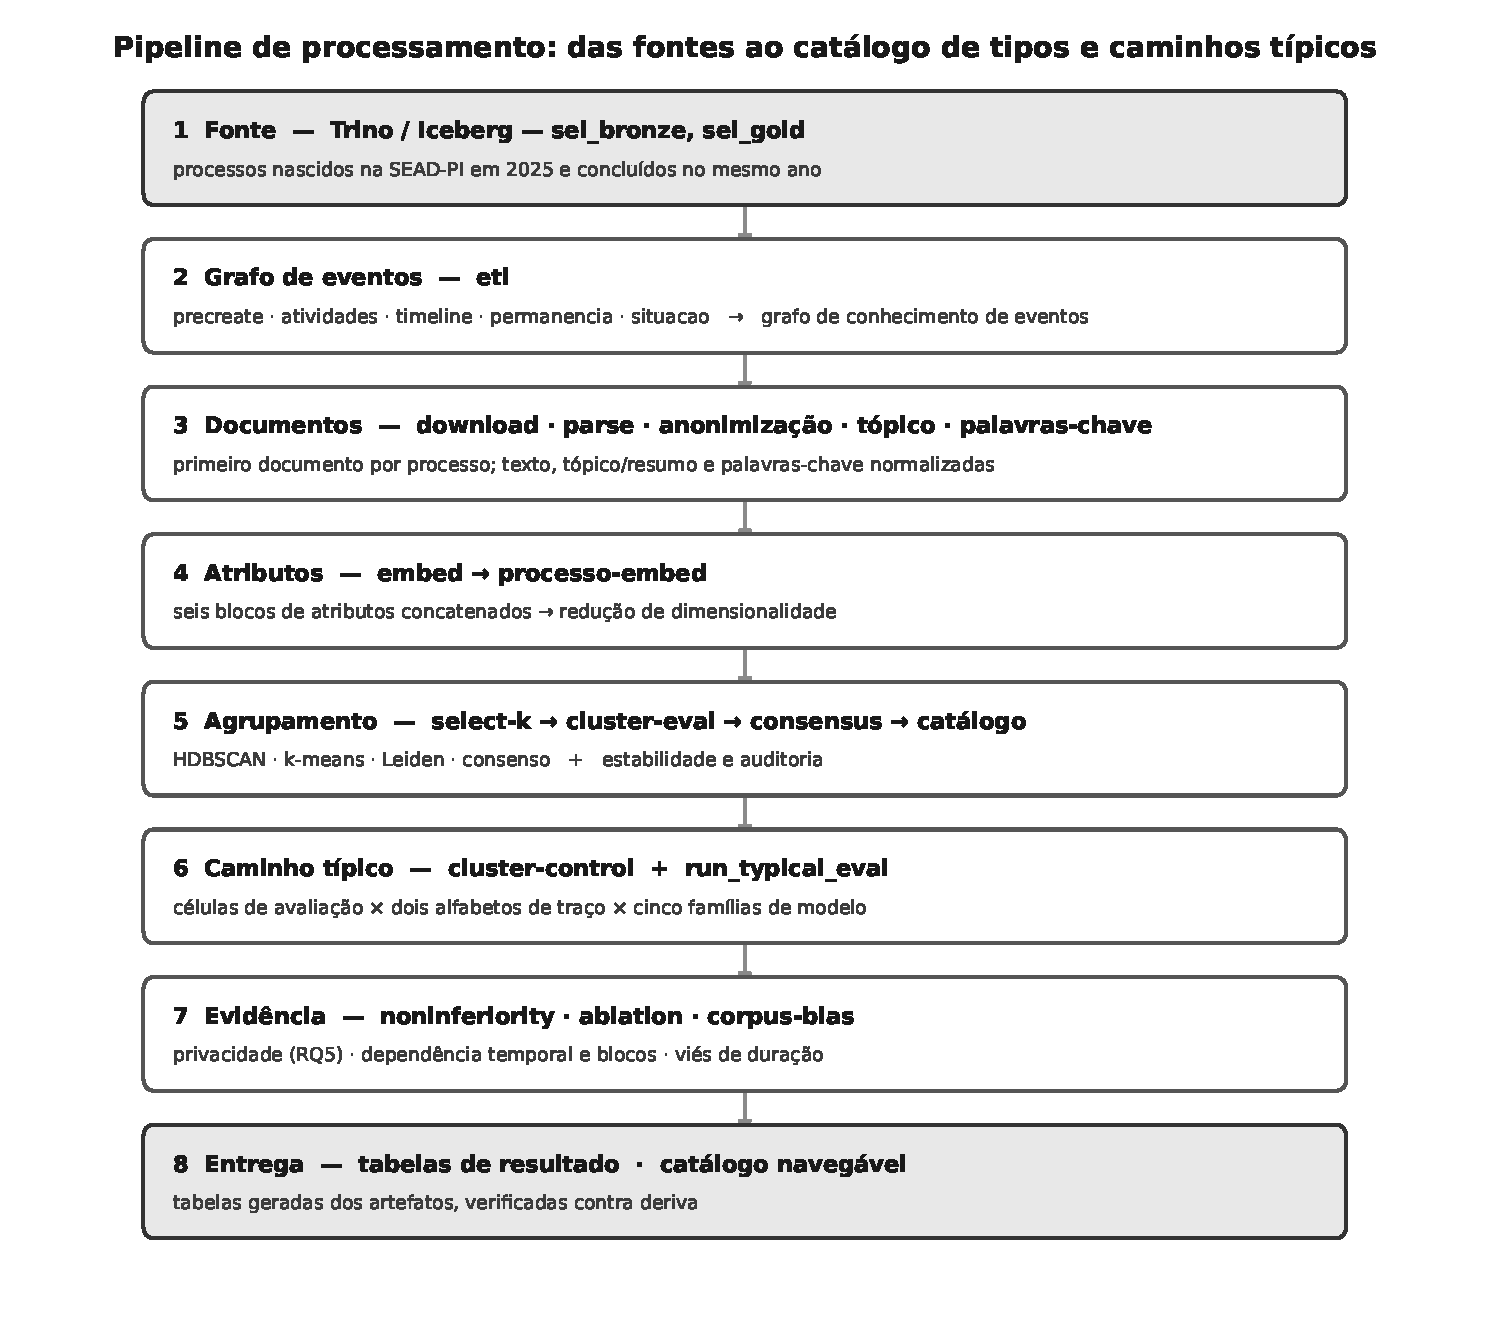
\includegraphics[width=\textwidth]{pipeline-macro.pdf}
\par\vspace{2pt}\footnotesize\raggedright O fluxo ilustra a sequência de extração, anonimização, vetorização, agrupamento e geração de caminhos típicos.
\end{figure}

\subsection{Caracterização da Pesquisa e Posicionalidade}\label{sec:caracterizacao}

Trata-se de uma pesquisa aplicada e quantitativa, caracterizada como estudo de caso único na SEAD-PI, com dados do ano de 2025. Conforme declarado na introdução, o vínculo funcional do autor com a secretaria exigiu a adoção de salvaguardas rigorosas (anonimização automatizada, processamento local e validação contra \emph{baselines} cegas) para evitar vieses e garantir o alinhamento com a autorização institucional de tratamento de dados \cite{seadpi2026termo}.

Neste texto, adota-se a seguinte convenção: \textbf{processo administrativo} refere-se ao caso individual analisado; \textbf{tipo de processo} é o agrupamento resultante (o \emph{cluster}); \textbf{traço} é a sequência de eventos de um processo; e \textbf{ação} é a tipologia do andamento registrado pelo sistema.

\subsection{Cenário, Corpus e Recorte Analítico}\label{sec:corpus}

O SEI não restringe as trajetórias dos processos administrativos. Embora as ações sigam ordem cronológica, um processo pode tramitar simultaneamente em múltiplas unidades. Para viabilizar a modelagem sequencial, este comportamento concorrente foi linearizado adotando-se a ordem cronológica estrita dos carimbos de tempo dos eventos.

Os dados foram extraídos do \emph{data lakehouse} da SEAD-PI (tabelas Iceberg via Trino). O recorte incluiu exclusivamente processos iniciados e concluídos na Secretaria no ano civil de 2025 que possuíam documento inicial legível. De 12.621 processos gerados, 5.445 foram carregados e \textbf{5.243} atenderam a todos os critérios e compõem o corpus da análise.

\subsubsection{Viés de Censura à Direita}\label{sec:vies}
Exigir a conclusão dentro do mesmo ano civil trunca a amostra, penalizando processos longos iniciados nos últimos meses do ano. Estimou-se um déficit de 18,2\% na população concluída, concentrado em trâmites prolongados. Consequentemente, o corpus não reflete durações médias globais de processamento, limitando inferências sobre eficiência temporal absoluta (Tabela~\ref{tab:corpus-bias}).

%% GENERATED by `pipeline run results` - do not edit by hand.
\begin{table}[htbp]
\centering
\caption{Censura à direita por mês de abertura.}\label{tab:corpus-bias}
\footnotesize
\begin{tabular}{lrrrrr}
\toprule
mês & observados & dias disponíveis & vida mediana & vida máxima & excl.\ estimada \\
\midrule
2025-01 & 474 & 365 & 21 & 343 & 0,0\% \\
2025-02 & 619 & 334 & 14 & 290 & 0,2\% \\
2025-03 & 478 & 306 & 17 & 284 & 0,8\% \\
2025-04 & 470 & 275 & 25 & 244 & 2,1\% \\
2025-05 & 415 & 245 & 24 & 225 & 5,1\% \\
2025-06 & 621 & 214 & 18 & 204 & 21,7\% \\
2025-07 & 653 & 184 & 12 & 166 & 24,1\% \\
2025-08 & 398 & 153 & 18 & 129 & 26,2\% \\
2025-09 & 539 & 122 & 10 & 105 & 29,3\% \\
2025-10 & 381 & 92 & 10 & 75 & 31,9\% \\
2025-11 & 268 & 61 & 5 & 42 & 35,9\% \\
2025-12 & 129 & 31 & 5 & 29 & 44,5\% \\
\bottomrule
\end{tabular}
\par\vspace{2pt}\footnotesize\raggedright Observados 5.445; verdadeiro estimado 6.658; ausentes estimados \textbf{1.213} (18,2\%). Limite inferior: o próprio mês de referência está truncado.
\end{table}


\subsection{Modelagem: Grafo de Conhecimento de Eventos}\label{sec:ekg}

Os \emph{logs} transacionais foram estruturados em um Grafo de Conhecimento de Eventos \cite{vanderaalst2016processmining, esser2021ekg}. A construção ocorreu em três etapas:
1. \textbf{Ingestão de Dimensões:} Criação de nós para unidades, usuários e tipos de procedimento.
2. \textbf{Anexação de Atividades:} Vinculação de cada atividade ao processo, unidade, usuário, ação e documento.
3. \textbf{Encadeamento Sequencial:} Conexão temporal das atividades do mesmo processo via relações de precedência direta.

A partir do grafo, derivaram-se as métricas de tempo de posse e retrabalho. Os traços gerados foram congelados em disco para isolar as fases de agrupamento e avaliação do banco de dados transacional.

\subsection{Processamento do Documento Inicial e Anonimização}\label{sec:documento}

Por exigência contratual da autorização de pesquisa \cite{seadpi2026termo}, a anonimização de dados pessoais antecedeu qualquer vetorização. O documento inicial foi convertido para texto plano (via extração nativa ou visão computacional local). Em seguida, aplicou-se uma dupla camada de detecção e supressão:
* \textbf{Mecanismos baseados em regras:} Validação de CPFs, CNPJs, e-mails e matrículas funcionais.
* \textbf{Reconhecimento de Entidades Nomeadas (NER):} Aplicação de um modelo neural de esquema aberto \cite{zaratiana2025gliner2} para substituir nomes próprios e informações sensíveis por marcadores consistentes (\emph{tokens} consistentes baseados no \emph{hash} da entidade, preservando a correferência).

A partir do texto limpo, um modelo de linguagem de pesos abertos gerou, para cada processo, um \textbf{tópico} e um \textbf{resumo} de uma frase, atuando como um filtro de ruído semântico. Além disso, extraiu-se um vocabulário controlado de palavras-chave através da unificação de n-gramas com similaridade de Dice $\geq 0,9$.

Para conformidade jurídica, toda inferência de rede neural foi executada no \emph{cluster} de alto desempenho local (Mandu, GPUs NVIDIA) do Governo do Estado do Piauí, sem chamadas a APIs externas.

\subsection{Vetorização e Agrupamento}\label{sec:atributos}

Cada processo administrativo foi representado pela concatenação de seis blocos de atributos, posteriormente reduzidos a 50 dimensões via UMAP \cite{mcinnes2018umap} (distância de cosseno):
1. \emph{Embeddings} do documento inicial (1.024 dimensões, via BGE-M3 \cite{chen2024bgem3}).
2. \emph{Embeddings} do tópico e resumo gerados (1.024 dimensões).
3. TF-IDF das unidades organizacionais visitadas (500 dimensões).
4. TF-IDF das transições entre unidades (1.000 dimensões).
5. Histograma de tipos de ações (48 dimensões).
6. TF-IDF das palavras-chave do documento (517 dimensões).

O agrupamento operou sobre esse espaço vetorial utilizando três famílias algorítmicas, varrendo hiperparâmetros para garantir robustez aos métodos: \textbf{HDBSCAN} (densidade) \cite{mcinnes2017hdbscan}, \textbf{K-means} (centroides) e \textbf{Leiden} (modularidade em grafos) \cite{traag2019leiden}. Essa grade gerou 14 configurações de clusterização (sete por braço: anonimizado vs. bruto). Processos não atribuídos pelo modelo de densidade (ruído) foram realocados ao centroide mais próximo para equalizar a população de avaliação entre os algoritmos.

\subsection{Alfabetos de Traço e Caminhos Típicos}\label{sec:caminhos}

A avaliação ocorreu separadamente sob três abstrações de alfabeto (Figura~\ref{fig:alfabetos}):

\begin{figure}[htbp]
\centering
% 1. O caption agora atua apenas como TÍTULO (conciso e direto)
\caption{Um mesmo processo administrativo renderizado nos três alfabetos de traço.}
\label{fig:alfabetos}

\fbox{\begin{minipage}{0.93\textwidth}
\vspace{2pt}
\raggedright\footnotesize
\textbf{Alfabeto de ação por unidade} --- excerto dos dezoito estados:

\vspace{2pt}
\texttt{GERACAO-PROCEDIMENTO@UNIDADE-A} · \texttt{GERACAO-DOCUMENTO@UNIDADE-A} ·
\texttt{ASSINATURA-DOCUMENTO@UNIDADE-A} · \texttt{CONCLUSAO-AUTOMATICA@UNIDADE-A} ·
\texttt{PROCESSO-REMETIDO@UNIDADE-B} · \texttt{PROCESSO-RECEBIDO@UNIDADE-B} ·
\texttt{GERACAO-DOCUMENTO@UNIDADE-B} · \ldots ·
\texttt{CONCLUSAO-PROCESSO@UNIDADE-A}

\vspace{6pt}
\textbf{Alfabeto de roteamento} --- os mesmos dezoito estados, colapsados em três:

\vspace{2pt}
\texttt{UNIDADE-A} $\rightarrow$ \texttt{UNIDADE-B} $\rightarrow$ \texttt{UNIDADE-A}

\vspace{6pt}
\textbf{Alfabeto de procedimento} --- os mesmos dezoito estados, abstraídos do organograma:

\vspace{2pt}
\texttt{GERACAO-PROCEDIMENTO} $\rightarrow$ \texttt{GERACAO-DOCUMENTO} $\rightarrow$
\texttt{ASSINATURA-DOCUMENTO} $\rightarrow$ \texttt{PROCESSO-REMETIDO} $\rightarrow$
\texttt{PROCESSO-RECEBIDO} $\rightarrow$ \texttt{GERACAO-DOCUMENTO} $\rightarrow$ \ldots
$\rightarrow$ \texttt{CONCLUSAO-PROCESSO}
\vspace{3pt}
\end{minipage}}

% 2. A legenda/nota explicativa vai para baixo, agrupando toda a explicação
\vspace{4pt}
\begin{minipage}{0.93\textwidth}
\footnotesize\justifying
\textbf{Nota:} O alfabeto de ação por unidade conserva o que se fez e onde; o de roteamento conserva apenas por onde o processo passou; o de procedimento conserva apenas o que se fez. Os dois últimos colapsam repetições consecutivas, avaliando populações distintas. A diferença central é a granularidade da representação: \texttt{ação@unidade} preserva localização, \texttt{roteamento} preserva trajetória e \texttt{procedimento} preserva ação.
\end{minipage}
\end{figure}

* \textbf{Ação por Unidade:} Estado completo não projetado (\emph{ação@unidade}).
* \textbf{Roteamento:} Sequência apenas das unidades organizacionais (foco organizacional).
* \textbf{Procedimento:} Sequência apenas das ações executadas (foco procedimental).

Para cada \emph{cluster} contendo ao menos 30 processos, ajustaram-se seis geradores sequenciais para predizer o próximo evento e compor o "caminho típico": Markov (3ª ordem), Grafo de Precedência Direta (DFG), GRU \cite{cho2014gru}, LSTM \cite{hochreiter1997lstm}, Transformer \cite{vaswani2017attention} e Redes Convolucionais em Grafos (GNN) \cite{kipf2017gcn}. Os hiperparâmetros das redes neurais foram fixados para evitar que a comparação capturasse apenas esforço de sintonia.

A geração foi submetida a uma decodificação restrita via máquina de estados, impedindo predições que violassem as regras sistêmicas de movimentação do SEI (ex: concluir um processo nunca recebido).

\subsection{Protocolo de Avaliação e Variáveis de Controle}\label{sec:protocolo}

Os processos foram particionados em 70\% (treino) e 30\% (teste). A métrica primária foi a \textbf{acurácia de próximo passo}, complementada por validações de sustentação de caminho (cobertura e suporte de transições observadas na realidade). 

Para isolar a qualidade da modelagem estrutural do mero "dividendo de partição" (facilidade inerente de prever vocabulários menores em grupos menores), utilizaram-se três linhas de base:
1. \textbf{Sucessor Intragrupo:} Predição pela frequência máxima de transição.
2. \textbf{Modelo Global:} Um único modelo (Markov 3ª ordem) treinado sobre todo o corpus.
3. \textbf{Partição Embaralhada:} Troca aleatória de rótulos dos processos, preservando tamanho e quantidade dos clusters, mas destruindo a pertinência semântica. 

O estimando principal ($\Delta^*$) consistiu na diferença de acurácia agregada ponderada entre a partição real proposta e a sua equivalente embaralhada. Uma partição cujo $\Delta^*$ não seja significativamente positivo foi considerada como não portadora de sinal latente útil.
\section{RESULTADOS E DISCUSSÃO}\label{sec:res}

Esta seção apresenta os resultados empíricos da aplicação do \emph{pipeline} sobre o corpus de 5.243 processos concluídos na SEAD-PI em 2025. A análise divide-se na avaliação do catálogo emergente frente à taxonomia oficial, no impacto dos atributos, na validação das partições via índices internos e no desempenho preditivo dos caminhos típicos. 

A avaliação foi estruturada em 14 agrupamentos, distribuídos por três alfabetos de traço (ação por unidade, roteamento e procedimento) e testados contra seis famílias de modelo, totalizando 84 células de avaliação, 4.323 grupos e 25.938 modelos treinados.

\subsection{O Catálogo Emergente vs. Taxonomia Declarada}\label{sec:res-catalogo}

O agrupamento dos 5.243 processos produziu entre 40 e 108 tipos ao longo das 14 configurações (com tamanho mediano variando de 39 a 94 processos). Nenhum processo ficou sem atribuição, visto que o ruído dos algoritmos de densidade foi realocado ao grupo mais próximo. A etapa de auditoria confirmou a regerabilidade exata (1,0) de todas as 14 partições a partir dos seus atributos.

Ao confrontar as partições emergentes com a taxonomia declarada pela administração, a concordância demonstrou-se moderada (Tabela~\ref{tab:taxonomy}). O Adjusted Rand Index (ARI) variou de 0,116 a 0,145 nos seis agrupamentos principais. 

%% GENERATED by `pipeline run results` - do not edit by hand.
\begin{table}[htbp]
\centering
\caption{Concordância entre a partição emergente e a taxonomia declarada.}\label{tab:taxonomy}
\footnotesize
\resizebox{\textwidth}{!}{%
\begin{tabular}{llrrrrr}
\toprule
agrupamento & escopo & $n$ & maioria & pureza & NMI & ARI \\
\midrule
exp-anon/hdbscan & todos & 5.243 & 0,302 & 0,730 & 0,530 & 0,145 \\
exp-anon/hdbscan & excl.\ genérica & 3.660 & 0,208 & 0,775 & 0,621 & 0,283 \\
exp-anon/kmeans & todos & 5.243 & 0,302 & 0,735 & 0,531 & 0,132 \\
exp-anon/kmeans & excl.\ genérica & 3.660 & 0,208 & 0,784 & 0,624 & 0,259 \\
exp-anon/leiden & todos & 5.243 & 0,302 & 0,727 & 0,521 & 0,116 \\
exp-anon/leiden & excl.\ genérica & 3.660 & 0,208 & 0,776 & 0,613 & 0,230 \\
exp-raw/hdbscan & todos & 5.243 & 0,302 & 0,728 & 0,527 & 0,138 \\
exp-raw/hdbscan & excl.\ genérica & 3.660 & 0,208 & 0,775 & 0,621 & 0,277 \\
exp-raw/kmeans & todos & 5.243 & 0,302 & 0,738 & 0,531 & 0,132 \\
exp-raw/kmeans & excl.\ genérica & 3.660 & 0,208 & 0,784 & 0,622 & 0,255 \\
exp-raw/leiden & todos & 5.243 & 0,302 & 0,723 & 0,524 & 0,120 \\
exp-raw/leiden & excl.\ genérica & 3.660 & 0,208 & 0,780 & 0,618 & 0,235 \\
\bottomrule
\end{tabular}
}
\end{table}


Essa discordância é impulsionada majoritariamente por uma única classe genérica ("documentos oficiais"), que abrange 30,2\% do corpus. Ao removê-la, o ARI salta para a faixa de 0,230 a 0,283. Para validar se o impacto advém do tamanho da classe ou de sua natureza, a Tabela~\ref{tab:catch-all-null} testa essa remoção contra uma hipótese nula pareada por volume. O resultado indica que remover partições aleatórias de tamanho equivalente degrada o ARI, confirmando que a taxonomia oficial perde precisão justamente por utilizar rótulos "guarda-chuva" de caráter arquivístico, em vez de capturar o fluxo procedimental real.

%% GENERATED by `pipeline run results` - do not edit by hand.
\begin{table}[htbp]
\centering
\caption{A classe genérica contra uma hipótese nula de classes aleatórias de mesmo tamanho.}\label{tab:catch-all-null}
\resizebox{\textwidth}{!}{%
\begin{tabular}{lrrrrrr}
\toprule
agrupamento & ARI total & ARI excl. & média nula & máx.\ nulo & $\geq$ obs. & $z$ \\
\midrule
exp-raw/hdbscan & 0,1383 & 0,2767 & 0,1010 $\pm$ 0,0189 & 0,1311 & 0/724 & 9,3 \\
exp-raw/kmeans & 0,1324 & 0,2548 & 0,0988 $\pm$ 0,0106 & 0,1231 & 0/724 & 14,8 \\
exp-raw/leiden & 0,1197 & 0,2348 & 0,0885 $\pm$ 0,0102 & 0,1076 & 0/724 & 14,3 \\
exp-anon/hdbscan & 0,1450 & 0,2831 & 0,1072 $\pm$ 0,0187 & 0,1375 & 0/724 & 9,4 \\
exp-anon/kmeans & 0,1317 & 0,2585 & 0,0974 $\pm$ 0,0110 & 0,1225 & 0/724 & 14,6 \\
exp-anon/leiden & 0,1161 & 0,2303 & 0,0851 $\pm$ 0,0102 & 0,1068 & 0/724 & 14,2 \\
\bottomrule
\end{tabular}
}
\par\vspace{2pt}\footnotesize\raggedright Nula: descartar um conjunto aleatório de classes declaradas inteiras somando até 10\% do tamanho da classe genérica e repontuar. Remover classes aleatórias do mesmo tamanho reduz a concordância; remover a classe genérica a aumenta. Nenhum sorteio nulo alcança o valor observado em qualquer agrupamento.
\end{table}


\subsection{Impacto dos Blocos de Atributos e Dependência Temporal}\label{sec:res-blocos}

A Tabela~\ref{tab:ablation} documenta o estudo de ablação realizado sobre o agrupamento por densidade (braço anonimizado). A remoção do bloco de palavras-chave reduz o ARI (0,596) a níveis comparáveis ao descarte de metade do histórico transacional de cada processo (0,649). Truncar a linha do tempo dos casos a 25\% reduz o ARI para 0,467, indicando que a caracterização precisa do processo se consolida no seu histórico de tramitação, e não apenas no documento de abertura.

%% GENERATED by `pipeline run results` - do not edit by hand.
\begin{table}[htbp]
\centering
\caption{Remoção controlada de blocos de atributos e de dependência temporal.}\label{tab:ablation}
\begin{tabular}{lrrr}
\toprule
variante & ARI & NMI & grupos \\
\midrule
Histórico truncado em 75\% & 0,798 & 0,895 & 68 \\
Histórico truncado em 50\% & 0,649 & 0,816 & 70 \\
Histórico truncado em 25\% & 0,467 & 0,717 & 53 \\
Bloco de palavras-chave removido & 0,596 & 0,838 & 65 \\
Bloco de tópicos removido & 0,840 & 0,905 & 71 \\
\bottomrule
\end{tabular}
\par\vspace{2pt}\footnotesize\raggedright Cada variante reconstrói os atributos sob uma única alteração e reagrupa; a concordância é medida contra a partição de histórico completo (64 grupos sobre 5.243 processos).
\end{table}


\subsubsection{Impacto da Estrutura Temporal na Classificação}\label{sec:res-holdout}

Para avaliar o quanto a estrutura temporal do processo afeta sua classificação e afastar a hipótese de que a predição possui alto desempenho apenas porque a partição agrupa processos com base em seu histórico tardio, os modelos foram testados contra agrupamentos construídos exclusivamente com os primeiros 25\% dos traços. A Tabela~\ref{tab:temporal-holdout} demonstra que no alfabeto de procedimento (o único onde a modelagem especializada supera consistentemente um modelo global), 92,5\% do ganho de acurácia sobrevive mesmo quando o agrupador ignora o futuro do processo. Nos demais alfabetos, o ganho aproxima-se do ruído residual, confirmando a robustez da classificação temporal e estrutural do método.

%% GENERATED by `pipeline run results` - do not edit by hand.
\begin{table}[htbp]
\centering
\caption{Ganho a jusante quando a partição vê apenas parte do histórico de cada processo.}\label{tab:temporal-holdout}
\resizebox{\textwidth}{!}{%
\begin{tabular}{lrrrrr}
\toprule
atributos do agrupamento & grupos & por grupo & global & ganho (como avaliado) & ganho (pareado) \\
\midrule
histórico completo & 41 & 0,6937 & 0,6856 & 0,0081 & \textbf{0,0097} \\
primeiros 75\% & 44 & 0,6942 & 0,6893 & 0,0049 & \textbf{0,0063} \\
primeiros 50\% & 46 & 0,6937 & 0,6940 & -0,0003 & \textbf{0,0040} \\
primeiros 25\% & 32 & 0,6777 & 0,6924 & -0,0147 & \textbf{-0,0057} \\
\bottomrule
\end{tabular}
}
\par\vspace{2pt}\footnotesize\raggedright Cada linha agrupa sobre atributos truncados em uma fração da linha do tempo de cada processo e então prevê sobre os traços retidos completos. As linhas não pareadas avaliam populações diferentes, de modo que seu gradiente reflete sobretudo o deslocamento da linha de base global; o bloco pareado repontua cada truncamento sobre os processos que todos os quatro avaliam. A última coluna repontua cada truncamento sobre os 1.091 processos que todos os quatro avaliam, que é a comparação que a coluna não pareada não consegue fazer.
\end{table}


\subsection{Diferenciação entre Partições e Índices Internos}\label{sec:res-particoes}

A exigência de tamanho mínimo (30 traços por grupo) e o colapso de repetições afetam a cobertura do corpus de maneira desigual. No alfabeto de roteamento, processos que tramitaram em uma única unidade perdem as transições e são descartados. Para equalizar a comparação entre as 14 configurações de agrupamento, todas foram repontuadas exclusivamente sobre o conjunto de 967 processos que sobrevivem aos cortes de todas elas (Tabela~\ref{tab:common-set}). A amplitude de acurácia observada entre a melhor e a pior partição foi de apenas \textbf{0,0055}, evidenciando que não há um agrupamento nitidamente superior com base exclusiva na acurácia preditiva.

%% GENERATED by `pipeline run results` - do not edit by hand.
\begin{table}[htbp]
\centering
\caption{Comparação entre agrupamentos sobre um conjunto comum de processos.}\label{tab:common-set}
\footnotesize
\begin{tabular}{lrrrr}
\toprule
agrupamento & $n$ próprio & conjunto próprio & conjunto comum & $\Delta$ \\
\midrule
exp-raw/leiden & 1.153 & 0,7107 & \textbf{0,7129} & 0,0022 \\
exp-raw-ksil/kmeans & 1.195 & 0,7081 & \textbf{0,7127} & 0,0046 \\
exp-anon/leiden & 1.122 & 0,7096 & \textbf{0,7114} & 0,0018 \\
exp-raw-kelbow/kmeans & 1.169 & 0,7126 & \textbf{0,7111} & -0,0015 \\
exp-raw-hcoarse/hdbscan & 1.207 & 0,7070 & \textbf{0,7109} & 0,0039 \\
exp-anon/hdbscan & 1.183 & 0,7054 & \textbf{0,7107} & 0,0053 \\
exp-anon-hcoarse/hdbscan & 1.199 & 0,7072 & \textbf{0,7101} & 0,0029 \\
exp-raw/hdbscan & 1.185 & 0,7030 & \textbf{0,7098} & 0,0068 \\
exp-anon/kmeans & 1.186 & 0,7058 & \textbf{0,7094} & 0,0036 \\
exp-raw-lres/leiden & 1.117 & 0,7046 & \textbf{0,7093} & 0,0047 \\
exp-anon-lres/leiden & 1.025 & 0,7049 & \textbf{0,7091} & 0,0042 \\
exp-raw/kmeans & 1.183 & 0,7067 & \textbf{0,7088} & 0,0021 \\
exp-anon-kelbow/kmeans & 1.170 & 0,7042 & \textbf{0,7074} & 0,0032 \\
exp-anon-ksil/kmeans & 1.195 & 0,7038 & \textbf{0,7074} & 0,0036 \\
\bottomrule
\end{tabular}
\par\vspace{2pt}\footnotesize\raggedright Todos os agrupamentos repontuados sobre os 967 processos que todos eles avaliam. Amplitude no conjunto comum: \textbf{0,0055}.
\end{table}


\subsubsection{Limitações dos Índices Internos de Validade}\label{sec:res-indices}

As Tabelas~\ref{tab:intrinsic-rows} e \ref{tab:intrinsic} reportam os índices internos de validação (Silhouette, DBCV, Davies-Bouldin, Calinski-Harabasz) e a utilidade a jusante. 

%% GENERATED by `pipeline run results` - do not edit by hand.
\begin{table}[htbp]
\centering
\caption{Índices internos de validade e qualidade a jusante, por agrupamento.}\label{tab:intrinsic-rows}
\resizebox{\textwidth}{!}{%
\begin{tabular}{lrrrrrrr}
\toprule
agrupamento & a jusante & DBCV & Silhouette & Davies--Bouldin & ruído & grupos & tamanho mediano \\
\midrule
exp-raw-kelbow/kmeans & 0,445 & -0,018 & 0,731 & 0,569 & 0,000 & 70 & 62 \\
exp-raw/leiden & 0,442 & 0,129 & 0,589 & 0,845 & 0,000 & 71 & 54 \\
exp-raw-lres/leiden & 0,426 & 0,094 & 0,647 & 0,807 & 0,000 & 98 & 51 \\
exp-raw/hdbscan & 0,411 & 0,018 & 0,688 & 0,861 & 0,000 & 66 & 60 \\
exp-anon/leiden & 0,405 & 0,064 & 0,546 & 0,932 & 0,000 & 75 & 54 \\
exp-anon-hcoarse/hdbscan & 0,399 & -0,075 & 0,573 & 0,733 & 0,000 & 40 & 94 \\
exp-anon-lres/leiden & 0,391 & 0,014 & 0,596 & 0,941 & 0,000 & 108 & 39 \\
exp-raw/kmeans & 0,391 & -0,012 & 0,737 & 0,539 & 0,000 & 66 & 64 \\
exp-raw-ksil/kmeans & 0,377 & -0,097 & 0,760 & 0,535 & 0,000 & 60 & 72 \\
exp-anon/hdbscan & 0,375 & -0,101 & 0,617 & 0,764 & 0,000 & 64 & 56 \\
exp-anon/kmeans & 0,372 & -0,066 & 0,732 & 0,586 & 0,000 & 64 & 75 \\
exp-raw-hcoarse/hdbscan & 0,371 & -0,075 & 0,662 & 0,748 & 0,000 & 42 & 80 \\
exp-anon-ksil/kmeans & 0,342 & -0,043 & 0,757 & 0,540 & 0,000 & 60 & 71 \\
exp-anon-kelbow/kmeans & 0,333 & -0,007 & 0,744 & 0,561 & 0,000 & 70 & 64 \\
\bottomrule
\end{tabular}
}
\par\vspace{2pt}\footnotesize\raggedright Uma linha por agrupamento, todas no mesmo espaço reduzido. As correlações da Tabela~\ref{tab:intrinsic} são calculadas sobre estas colunas. A taxa de ruído é a parcela de processos que o algoritmo deixa sem atribuição; os métodos por densidade são os únicos em que ela é diferente de zero.
\end{table}

%% GENERATED by `pipeline run results` - do not edit by hand.
\begin{table}[htbp]
\centering
\caption{Índices internos de validade contra a utilidade a jusante.}\label{tab:intrinsic}
\begin{tabular}{lrr}
\toprule
índice & $\rho$ & $p$ \\
\midrule
DBCV & 0,538 & 0,053 \\
Silhouette & -0,516 & 0,060 \\
Davies--Bouldin & 0,464 & 0,100 \\
Calinski--Harabasz & -0,270 & 0,354 \\
Taxa de ruído (recusada) & -0,055 & 0,853 \\
Número de grupos & 0,501 & 0,073 \\
Tamanho mediano de grupo & -0,524 & 0,061 \\
\bottomrule
\end{tabular}
\par\vspace{2pt}\footnotesize\raggedright Correlação de postos de Spearman com a qualidade a jusante em 14 agrupamentos; teste de permutação com 20.000 sorteios. A medida a jusante abrange 0,112 (34\% relativo).
\end{table}


Nenhum dos oito índices geométricos testados conseguiu prever de forma confiável a utilidade final dos caminhos típicos gerados (o menor $p$-valor sob permutação foi 0,053 para o DBCV). Métricas clássicas de compacidade, como DBCV e Silhouette, correlacionaram-se com a predição a jusante em sentidos opostos. A Tabela~\ref{tab:index-mechanism} demonstra que a forte correlação dos índices restringe-se apenas a características dimensionais, como o número de grupos (granularidade), e não à fidelidade comportamental. Por consequência, a seleção do modelo a ser publicado não deve ser delegada cegamente a métricas internas.

%% GENERATED by `pipeline run results` - do not edit by hand.
\begin{table}[htbp]
\centering
\caption{O que os índices de validade de fato acompanham.}\label{tab:index-mechanism}
\footnotesize
\begin{tabular}{lll}
\toprule
relação & população & $\rho$ \\
\midrule
Silhouette vs.\ parcela de processos descartados como ruído & todos os 14 & -0,308 \\
Parcela descartada vs.\ acurácia no conjunto próprio da partição & todos os 14 & -0,204 \\
Silhouette vs.\ tamanho mediano de grupo & cob.\ total 14 & 0,427 \\
Silhouette vs.\ número de grupos & cob.\ total 14 & -0,325 \\
Número de grupos vs.\ cobertura & cob.\ total 14 & -0,991 \\
Silhouette vs.\ cobertura & cob.\ total 14 & 0,341 \\
\textbf{Silhouette vs.\ acurácia no conjunto comum} & cob.\ total 14 & \textbf{-0,392} \\
\textbf{DBCV vs.\ acurácia no conjunto comum} & cob.\ total 14 & \textbf{-0,057} \\
Silhouette vs.\ acurácia, apenas grupos pequenos (top-1 médio 0,623) & 233 grupos, 14 valores & -0,151 \\
Silhouette vs.\ acurácia, apenas grupos médios (top-1 médio 0,655) & 267 grupos, 14 valores & -0,009 \\
Silhouette vs.\ acurácia, apenas grupos grandes (top-1 médio 0,781) & 89 grupos, 14 valores & 0,074 \\
\bottomrule
\end{tabular}
\par\vspace{2pt}\footnotesize\raggedright A granularidade é a relação que resiste ao escrutínio neste tamanho de amostra. As linhas de cobertura são em grande medida uma reformulação dela (a correlação parcial dado o tamanho mediano de grupo é pequena), e a diferença entre as correlações de cobertura e de acurácia não é resolvível aqui -- seu intervalo bootstrap sobre as configurações inclui zero. As linhas de faixa carregam apenas tantos valores distintos de silhouette quantas são as partições, e não quantos são os grupos, de modo que constituem evidência muito mais fraca do que suas contagens de grupos sugerem.
\end{table}


\subsection{Avaliação Preditiva contra Linhas de Base}\label{sec:res-caminhos}

A capacidade preditiva das seis famílias de modelos foi submetida a 252 comparações contra controles estritos (Tabelas~\ref{tab:controls}, \ref{tab:delta-star}). 

\subsubsection{Comparação contra Partições Embaralhadas (\texorpdfstring{$\Delta^*$}{Delta*})}\label{sec:res-sinal}

Para isolar o valor informacional do agrupamento em relação ao mero "dividendo de partição" (facilidade de prever classes em vocabulários menores), utilizou-se a métrica $\Delta^*$: a diferença de acurácia entre a partição real e uma versão com os mesmos tamanhos e populações, porém com a pertinência dos rótulos embaralhada.

O $\Delta^*$ mostrou-se positivo em \textbf{100\% das 252 comparações}. No alfabeto de ação por unidade, atingiu de 0,165 a 0,328; em roteamento, de 0,143 a 0,285; e em procedimento, de 0,119 a 0,177. A pertença aos grupos carrega, portanto, um sinal estrutural latente válido que a taxonomia oficial não reflete. 

%% GENERATED by `pipeline run results` - do not edit by hand.
\begin{table}[htbp]
\centering
\caption{Acurácia do próximo passo contra três linhas de base, alfabeto de ação por unidade.}\label{tab:controls}
\label{tab:controls-unit}
\resizebox{\textwidth}{!}{%
\begin{tabular}{rrrrrrrrr}
\toprule
melhor sel. & sucessor & global & embaralhado & $\Delta$ família fixa & $\Delta$ melhor família & F1 de arestas & F1 de arestas embaralhado & $\Delta^{*}$ F1 de arestas \\
\midrule
0,722 & 0,632 & 0,712 & 0,512 & \textbf{0,000} & 0,003 & 0,501 & 0,361 & 0,140 \\
\bottomrule
\end{tabular}
}
\par\vspace{2pt}\footnotesize\raggedright ``melhor selecionado'' toma o máximo por grupo sobre todas as famílias de modelo, de modo que o seu ganho sobre uma linha de base global de família única não é termo a termo; as colunas $\Delta$ mantêm a família fixa. $\Delta$ ainda contém o que uma partição desta distribuição de tamanhos obtém por si só, razão pela qual a coluna embaralhada é reportada ao lado e a contribuição própria da partição é separada na sua própria tabela. edge-F1 é a média harmônica entre a cobertura de arestas de precedência direta e o seu uso; é uma estatística de grupo e não uma saída de modelo, logo assume um único valor por partição e não pode variar por família de modelo. Todo número é medido dentro de um alfabeto, contra uma linha de base que enfrenta o mesmo vocabulário; os alfabetos nunca são tabulados em conjunto, porque acurácias sobre vocabulários de tamanhos diferentes não são a mesma grandeza.
\end{table}

\begin{table}[htbp]
\centering
\caption{Acurácia do próximo passo contra três linhas de base, alfabeto de roteamento.}\label{tab:controls-itinerary}
\resizebox{\textwidth}{!}{%
\begin{tabular}{rrrrrrrrr}
\toprule
melhor sel. & sucessor & global & embaralhado & $\Delta$ família fixa & $\Delta$ melhor família & F1 de arestas & F1 de arestas embaralhado & $\Delta^{*}$ F1 de arestas \\
\midrule
0,721 & 0,481 & 0,689 & 0,517 & \textbf{0,010} & 0,023 & 0,545 & 0,425 & 0,120 \\
\bottomrule
\end{tabular}
}
\par\vspace{2pt}\footnotesize\raggedright ``melhor selecionado'' toma o máximo por grupo sobre todas as famílias de modelo, de modo que o seu ganho sobre uma linha de base global de família única não é termo a termo; as colunas $\Delta$ mantêm a família fixa. $\Delta$ ainda contém o que uma partição desta distribuição de tamanhos obtém por si só, razão pela qual a coluna embaralhada é reportada ao lado e a contribuição própria da partição é separada na sua própria tabela. edge-F1 é a média harmônica entre a cobertura de arestas de precedência direta e o seu uso; é uma estatística de grupo e não uma saída de modelo, logo assume um único valor por partição e não pode variar por família de modelo. Todo número é medido dentro de um alfabeto, contra uma linha de base que enfrenta o mesmo vocabulário; os alfabetos nunca são tabulados em conjunto, porque acurácias sobre vocabulários de tamanhos diferentes não são a mesma grandeza.
\end{table}

\begin{table}[htbp]
\centering
\caption{Acurácia do próximo passo contra três linhas de base, alfabeto de ação.}\label{tab:controls-procedure}
\resizebox{\textwidth}{!}{%
\begin{tabular}{rrrrrrrrr}
\toprule
melhor sel. & sucessor & global & embaralhado & $\Delta$ família fixa & $\Delta$ melhor família & F1 de arestas & F1 de arestas embaralhado & $\Delta^{*}$ F1 de arestas \\
\midrule
0,760 & 0,649 & 0,624 & 0,607 & \textbf{0,109} & 0,131 & 0,729 & 0,734 & -0,006 \\
\bottomrule
\end{tabular}
}
\par\vspace{2pt}\footnotesize\raggedright ``melhor selecionado'' toma o máximo por grupo sobre todas as famílias de modelo, de modo que o seu ganho sobre uma linha de base global de família única não é termo a termo; as colunas $\Delta$ mantêm a família fixa. $\Delta$ ainda contém o que uma partição desta distribuição de tamanhos obtém por si só, razão pela qual a coluna embaralhada é reportada ao lado e a contribuição própria da partição é separada na sua própria tabela. edge-F1 é a média harmônica entre a cobertura de arestas de precedência direta e o seu uso; é uma estatística de grupo e não uma saída de modelo, logo assume um único valor por partição e não pode variar por família de modelo. Todo número é medido dentro de um alfabeto, contra uma linha de base que enfrenta o mesmo vocabulário; os alfabetos nunca são tabulados em conjunto, porque acurácias sobre vocabulários de tamanhos diferentes não são a mesma grandeza.
\end{table}

%% GENERATED by `pipeline run results` - do not edit by hand.
\begin{table}[htbp]
\centering
\caption{Contribuição da própria partição, alfabeto de ação por unidade.}\label{tab:delta-star}
\label{tab:delta-star-unit}
\resizebox{\textwidth}{!}{%
\begin{tabular}{lrrrrr}
\toprule
família & top-1 real & top-1 embaralhado & $\Delta^{*}$ top-1 & $\Delta^{*}$ ajustado & $\Delta^{*}$ cobertura \\
\midrule
markov & 0,712 & 0,508 & \textbf{0,204} & 0,186 & 0,088 \\
gru & 0,715 & 0,496 & \textbf{0,219} & 0,202 & 0,118 \\
lstm & 0,705 & 0,471 & \textbf{0,234} & 0,216 & 0,121 \\
transformer & 0,713 & 0,488 & \textbf{0,225} & 0,207 & 0,154 \\
gnn & 0,625 & 0,428 & \textbf{0,197} & 0,179 & 0,073 \\
dfg & 0,589 & 0,296 & \textbf{0,293} & 0,275 & 0,095 \\
\bottomrule
\end{tabular}
}
\par\vspace{2pt}\footnotesize\raggedright $\Delta^{*}$ é o estimando: a partição real menos o seu controle embaralhado de forma equivalente, que tem o mesmo número de grupos, a mesma distribuição de tamanhos e a mesma população, com a pertença permutada. Ajustar um modelo por família muda o que esse modelo vê, de modo que uma partição desta forma desloca a acurácia por si só; apenas o excesso sobre o controle é atribuível ao agrupamento. $\Delta^{*}$ ajustado subtrai adicionalmente o modelo global agregado sob ambas as partições, cancelando um pequeno artefato de ponderação. $\Delta^{*}$ cobertura aplica o mesmo contraste a revocação de unidades $\times$ top-1 $/(1+$transições não vistas$)$. $\Delta^{*}$ é um critério de admissão, não uma ordenação: cresce com o número de famílias, porque especializar compensa mais quando as famílias são pequenas, de modo que partições de granularidade diferente não devem ser ordenadas por ele. Os alfabetos nunca são tabulados em conjunto.
\end{table}

\begin{table}[htbp]
\centering
\caption{Contribuição da própria partição, alfabeto de roteamento.}\label{tab:delta-star-itinerary}
\begin{tabular}{lrrrrr}
\toprule
família & top-1 real & top-1 embaralhado & $\Delta^{*}$ top-1 & $\Delta^{*}$ ajustado & $\Delta^{*}$ cobertura \\
\midrule
markov & 0,698 & 0,507 & \textbf{0,191} & 0,176 & 0,337 \\
gru & 0,705 & 0,485 & \textbf{0,220} & 0,205 & 0,339 \\
lstm & 0,690 & 0,448 & \textbf{0,242} & 0,227 & 0,290 \\
transformer & 0,711 & 0,499 & \textbf{0,212} & 0,198 & 0,306 \\
gnn & 0,477 & 0,304 & \textbf{0,173} & 0,158 & 0,174 \\
dfg & 0,460 & 0,261 & \textbf{0,200} & 0,185 & 0,191 \\
\bottomrule
\end{tabular}
\par\vspace{2pt}\footnotesize\raggedright $\Delta^{*}$ é o estimando: a partição real menos o seu controle embaralhado de forma equivalente, que tem o mesmo número de grupos, a mesma distribuição de tamanhos e a mesma população, com a pertença permutada. Ajustar um modelo por família muda o que esse modelo vê, de modo que uma partição desta forma desloca a acurácia por si só; apenas o excesso sobre o controle é atribuível ao agrupamento. $\Delta^{*}$ ajustado subtrai adicionalmente o modelo global agregado sob ambas as partições, cancelando um pequeno artefato de ponderação. $\Delta^{*}$ cobertura aplica o mesmo contraste a revocação de unidades $\times$ top-1 $/(1+$transições não vistas$)$. $\Delta^{*}$ é um critério de admissão, não uma ordenação: cresce com o número de famílias, porque especializar compensa mais quando as famílias são pequenas, de modo que partições de granularidade diferente não devem ser ordenadas por ele. Os alfabetos nunca são tabulados em conjunto.
\end{table}

\begin{table}[htbp]
\centering
\caption{Contribuição da própria partição, alfabeto de ação.}\label{tab:delta-star-procedure}
\begin{tabular}{lrrrr}
\toprule
família & top-1 real & top-1 embaralhado & $\Delta^{*}$ top-1 & $\Delta^{*}$ ajustado \\
\midrule
markov & 0,733 & 0,587 & \textbf{0,146} & 0,152 \\
gru & 0,755 & 0,601 & \textbf{0,153} & 0,160 \\
lstm & 0,754 & 0,599 & \textbf{0,155} & 0,161 \\
transformer & 0,751 & 0,593 & \textbf{0,158} & 0,165 \\
gnn & 0,644 & 0,515 & \textbf{0,129} & 0,136 \\
dfg & 0,644 & 0,517 & \textbf{0,126} & 0,133 \\
\bottomrule
\end{tabular}
\par\vspace{2pt}\footnotesize\raggedright $\Delta^{*}$ é o estimando: a partição real menos o seu controle embaralhado de forma equivalente, que tem o mesmo número de grupos, a mesma distribuição de tamanhos e a mesma população, com a pertença permutada. Ajustar um modelo por família muda o que esse modelo vê, de modo que uma partição desta forma desloca a acurácia por si só; apenas o excesso sobre o controle é atribuível ao agrupamento. $\Delta^{*}$ ajustado subtrai adicionalmente o modelo global agregado sob ambas as partições, cancelando um pequeno artefato de ponderação. $\Delta^{*}$ cobertura aplica o mesmo contraste a revocação de unidades $\times$ top-1 $/(1+$transições não vistas$)$. $\Delta^{*}$ é um critério de admissão, não uma ordenação: cresce com o número de famílias, porque especializar compensa mais quando as famílias são pequenas, de modo que partições de granularidade diferente não devem ser ordenadas por ele. Os alfabetos nunca são tabulados em conjunto.
\end{table}


Contudo, observou-se que o $\Delta^*$ cresce monotonicamente junto com a granularidade dos agrupamentos: grupos menores geram controles embaralhados mais fracos. Portanto, o $\Delta^*$ atua como um teste de admissibilidade estatística (comprova que há padrão), e não como uma função de ordenação para eleger a melhor partição candidata.

\subsubsection{Desempenho das Famílias de Modelos e Fidelidade de Arestas}\label{sec:res-familias}

A diferença de desempenho preditivo entre modelos estocásticos clássicos e arquiteturas neurais complexas foi marginal nos três alfabetos. No alfabeto de roteamento, a cadeia de Markov de 3ª ordem alcançou 0,698 de acurácia, ficando a apenas 1,3 ponto percentual do Transformer (0,711). No alfabeto de procedimento, a cadeia de Markov marcou 0,733 contra 0,754 da arquitetura GRU (diferença de 2,2 pontos). Esses resultados indicam que modelos de menor custo computacional (baseados em matrizes de transição) entregam resultados competitivos frente a redes neurais neste domínio específico.

A métrica de fidelidade de arestas (Edge-F1), que avalia a topologia do grafo gerado, revelou que o ganho preditivo de próximo passo não se traduz necessariamente em ganho estrutural. No alfabeto de procedimento, o Edge-F1 da partição real foi 0,729 contra 0,734 do controle embaralhado ($\Delta^* = -0{,}006$). Isso demonstra que o valor do particionamento, neste caso, incide sobre a previsão da sequência linear de ações (o modelo de linguagem do traço), e não sobre a descoberta de fluxos de trabalho estruturalmente distintos.

\subsubsection{Estratificação por Tamanho de Grupo e Comparação com Processos Reais}\label{sec:res-tamanho}

O desempenho dos modelos foi estratificado pelo número de instâncias contidas em cada \emph{cluster}. Conforme detalhado nas tabelas de tendência por tamanho, grupos maiores tendem a gerar caminhos preditivos com menor taxa de fabricação de transições inéditas, especialmente nos alfabetos de roteamento e ação por unidade. 

%% GENERATED by `pipeline run results` - do not edit by hand.
\begin{table}[htbp]
\centering
\caption{Qualidade do caminho por tamanho de grupo, alfabeto de ação por unidade.}\label{tab:size-trend-unit}
\resizebox{\textwidth}{!}{%
\begin{tabular}{lrrrrr}
\toprule
processos no grupo & grupos & top-1 & ganho vs global & revocação de unidades & inéditas \\
\midrule
30-50 & 183 & 0,669 & 0,0047 & 0,705 & 8,154 \\
50-75 & 232 & 0,693 & 0,0062 & 0,643 & 2,581 \\
75-100 & 130 & 0,669 & -0,0015 & 0,650 & 3,401 \\
100-150 & 109 & 0,725 & 0,0170 & 0,711 & 3,273 \\
150-250 & 85 & 0,762 & 0,0108 & 0,774 & 1,331 \\
250- & 25 & 0,817 & 0,0283 & 0,795 & 0,252 \\
\bottomrule
\end{tabular}
}
\par\vspace{2pt}\footnotesize\raggedright O ganho é medido faixa a faixa contra um modelo global da mesma família. Grupos com menos de trinta traços não são avaliados.
\end{table}

\begin{table}[htbp]
\centering
\caption{Qualidade do caminho por tamanho de grupo, alfabeto de roteamento.}\label{tab:size-trend-itinerary}
\footnotesize
\resizebox{\textwidth}{!}{%
\begin{tabular}{lrrrrr}
\toprule
processos no grupo & grupos & top-1 & ganho vs global & revocação de unidades & inéditas \\
\midrule
30-50 & 157 & 0,668 & 0,0361 & 0,737 & 1,226 \\
50-75 & 148 & 0,657 & 0,0264 & 0,648 & 0,554 \\
75-100 & 111 & 0,665 & 0,0543 & 0,670 & 0,470 \\
100-150 & 84 & 0,719 & 0,0383 & 0,702 & 0,393 \\
150-250 & 70 & 0,782 & 0,0172 & 0,811 & 0,268 \\
250- & 19 & 0,830 & 0,0257 & 0,797 & 0,103 \\
\bottomrule
\end{tabular}
}
\par\vspace{2pt}\footnotesize\raggedright O ganho é medido faixa a faixa contra um modelo global da mesma família. Grupos com menos de trinta traços não são avaliados.
\end{table}

\begin{table}[htbp]
\centering
\caption{Qualidade do caminho por tamanho de grupo, alfabeto de ação.}\label{tab:size-trend-procedure}
\footnotesize
\resizebox{\textwidth}{!}{%
\begin{tabular}{lrrrr}
\toprule
processos no grupo & grupos & top-1 & ganho vs global & inéditas \\
\midrule
30-50 & 183 & 0,721 & 0,1092 & 4,215 \\
50-75 & 232 & 0,743 & 0,1340 & 1,794 \\
75-100 & 130 & 0,718 & 0,1229 & 1,990 \\
100-150 & 109 & 0,757 & 0,1313 & 2,675 \\
150-250 & 85 & 0,793 & 0,1450 & 2,817 \\
250- & 25 & 0,827 & 0,1797 & 5,155 \\
\bottomrule
\end{tabular}
}
\par\vspace{2pt}\footnotesize\raggedright O ganho é medido faixa a faixa contra um modelo global da mesma família. Grupos com menos de trinta traços não são avaliados.
\end{table}


Para avaliar o grau de realismo das predições, os caminhos gerados foram confrontados com o medoide (o traço real mais central de cada grupo). Constatou-se uma subgeração sistemática: os caminhos sintéticos cobrem apenas cerca de 52\% a 54\% das visitas de um processo real e são estruturalmente mais curtos. No alfabeto de roteamento, os modelos generativos (como Markov e GRU) produziram rotas mais "limpas" (menos idiossincráticas e com menor fabricação de arestas) que o próprio medoide. No alfabeto de procedimento, entretanto, o medoide superou todos os geradores sintéticos ao apresentar uma fabricação quase nula de arestas inéditas (0,415 transições não observadas, contra 2,993 da GRU).

\subsection{Conformidade com as Regras de Tramitação}\label{sec:res-conformidade}

A viabilidade técnica de um catálogo auditável exige que os caminhos gerados não violem as lógicas fundamentais do sistema de origem. A Tabela~\ref{tab:flow} consolida os testes de conformidade em relação às regras de pareamento (envio e recebimento) do SEI.

%% GENERATED by `pipeline run results` - do not edit by hand.
\begin{table}[htbp]
\centering
\caption{Conformidade às regras na geração irrestrita, comparada aos próprios registros de atividades.}\label{tab:flow}
\footnotesize
\resizebox{0.85\textwidth}{!}{%
\begin{tabular}{lrr}
\toprule
fonte & passos válidos & traços totalmente válidos \\
\midrule
markov & 0,9978 & 0,9486 \\
dfg & 0,9934 & 0,9337 \\
gnn & 0,9869 & 0,8756 \\
gru & 0,9930 & 0,8894 \\
lstm & 0,9908 & 0,8639 \\
transformer & 0,9900 & 0,8719 \\
\emph{registros de atividades reais} & 0,9986 & 0,9162 \\
\bottomrule
\end{tabular}
}
\par\vspace{2pt}\footnotesize\raggedright A decodificação restrita é válida por construção e não é tabulada.
\end{table}


No alfabeto de ação por unidade, a geração irrestrita obteve alta aderência: entre 86,4\% e 94,9\% dos traços gerados respeitaram nativamente as regras de fluxo. No entanto, no alfabeto de procedimento, as próprias instâncias reais violam a regra em larga escala (apenas 24,40\% de conformidade no log original). A aplicação da decodificação restrita via máquina de estados mitigou esse problema, garantindo a validade estrutural por construção ao custo de alterar o candidato preditivo ótimo em cerca de 1,07\% das decisões de roteamento.

\subsection{Anonimização e Custo de Utilidade}\label{sec:res-anon}

O impacto da supressão de dados pessoais (exigida pela LGPD e pelo termo de autorização) sobre a acurácia preditiva foi avaliado comparando-se o braço bruto e o braço anonimizado processo a processo, via \emph{bootstrap} pareado com 2.000 replicações. 

Os resultados mostram que todas as 54 comparações de modelo por agrupamento foram não inferiores na margem pré-registrada $\delta = 0{,}01$. Sob a margem de sensibilidade mais restrita de $\delta = 0{,}005$, obteve-se sucesso em 49 das 54 medições. Conclui-se que a anonimização textual aplicada previamente não impõe custo estatisticamente relevante à utilidade preditiva a jusante.

\subsection{Seleção da Configuração do Catálogo Final}\label{sec:selecao}

Como a amplitude de acurácia entre as 14 partições sobre o conjunto comum foi estatisticamente mínima (0,0055) e os índices geométricos internos demonstraram-se falhos para ordenação, a seleção da partição final exigiu critérios heurísticos alinhados ao objetivo do artefato de transparência.

A Tabela~\ref{tab:selection} ilustra a pontuação dos candidatos baseada na composição de cobertura, tamanho mediano, acurácia e \emph{silhouette}.

%% GENERATED by `pipeline run results` - do not edit by hand.
\begin{table}[htbp]
\centering
\caption{Escolha de um entregável entre os agrupamentos, pontuada apenas no alfabeto de roteamento.}\label{tab:selection}
\footnotesize
\resizebox{\textwidth}{!}{%
\begin{tabular}{lrrrrrrr}
\toprule
agrupamento & t-1 comum & cobertura & silh. & tam.\ mediano & grupos & em grupos $\ge$150 & escore \\
\midrule
exp-raw-ksil/kmeans & 0,7127 & 0,751 & 0,760 & 72 & 60 & 0,324 & \textbf{0,900} \\
exp-raw-hcoarse/hdbscan & 0,7109 & 0,759 & 0,662 & 80 & 42 & 0,631 & \textbf{0,746} \\
exp-raw-kelbow/kmeans & 0,7111 & 0,735 & 0,731 & 62 & 70 & 0,310 & \textbf{0,689} \\
exp-raw/leiden & 0,7129 & 0,727 & 0,589 & 54 & 71 & 0,331 & \textbf{0,676} \\
exp-anon-hcoarse/hdbscan & 0,7101 & 0,757 & 0,573 & 94 & 40 & 0,680 & \textbf{0,658} \\
exp-anon/kmeans & 0,7094 & 0,747 & 0,732 & 75 & 64 & 0,331 & \textbf{0,639} \\
exp-anon/hdbscan & 0,7107 & 0,745 & 0,617 & 56 & 64 & 0,363 & \textbf{0,594} \\
exp-raw/hdbscan & 0,7098 & 0,744 & 0,688 & 60 & 66 & 0,345 & \textbf{0,588} \\
exp-raw/kmeans & 0,7088 & 0,741 & 0,737 & 64 & 66 & 0,321 & \textbf{0,551} \\
exp-anon-ksil/kmeans & 0,7074 & 0,752 & 0,757 & 71 & 60 & 0,338 & \textbf{0,513} \\
exp-anon/leiden & 0,7114 & 0,711 & 0,546 & 54 & 75 & 0,267 & \textbf{0,491} \\
exp-anon-kelbow/kmeans & 0,7074 & 0,734 & 0,744 & 64 & 70 & 0,178 & \textbf{0,432} \\
exp-raw-lres/leiden & 0,7093 & 0,698 & 0,647 & 51 & 98 & 0,040 & \textbf{0,363} \\
exp-anon-lres/leiden & 0,7091 & 0,656 & 0,596 & 39 & 108 & 0,033 & \textbf{0,159} \\
\bottomrule
\end{tabular}
}
\par\vspace{2pt}\footnotesize\raggedright Todo agrupamento é candidato: nenhum filtro de cobertura é aplicado, uma vez que atribuir o ruído da densidade ao grupo mais próximo já fechou o canal de descarte a montante. Os atributos são escalonados por mín--máx entre os candidatos; a acurácia é pontuada sobre o conjunto comum. Pontuado apenas no alfabeto de roteamento --- os alfabetos nunca são agregados entre si, de modo que o entregável é selecionado sobre um deles, e essa escolha é uma decisão de escopo, e não uma propriedade dos dados. O mesmo candidato vence sob todas as quatro ponderações, inclusive uma que ignora inteiramente os índices de validade. ``em grupos $\ge$150'' é a fração de processos que a partição situa em grupos grandes o bastante para a faixa de baixa fabricação da Tabela~\ref{tab:size-trend-itinerary}.
\end{table}


A configuração selecionada para a entrega metodológica foi o \textbf{agrupamento por centroides (K-means) do braço sem anonimização com $k$ definido pela \emph{silhouette}}. Essa parametrização assegura a formação de 60 grupos com um tamanho mediano robusto (71,5 processos) e 75,1\% de cobertura do corpus avaliável. A geração dos caminhos típicos foi parametrizada utilizando a arquitetura \textbf{GRU} sob o alfabeto de \textbf{roteamento}, priorizando a interpretabilidade organizacional exigida por relatórios de conformidade pública.

\subsection{Estrutura do Catálogo Entregue}\label{sec:res-entrada}

Com a configuração final estabelecida, a Tabela~\ref{tab:catalogue} ilustra dez das 60 entradas nomeadas que compõem o artefato entregue. A tabela evidencia a dispersão intrínseca na qualidade de predição entre diferentes tipos processuais: categorias estruturadas, como "alterações contratuais" (210 processos), atingem 0,984 de acurácia de próximo passo; em contraste, agrupamentos mais difusos, como o de "justificativa de ponto", apresentam acurácia na faixa de 0,570. Por essa razão, as métricas de suporte e o tamanho do grupo devem obrigatoriamente acompanhar a publicação de cada entrada no catálogo real.

%% GENERATED by `pipeline run results` - do not edit by hand.
\begin{table}[htbp]
\centering
\caption{Entradas ilustrativas do catálogo: os maiores e os menores tipos avaliados.}\label{tab:catalogue}
\footnotesize
\resizebox{\textwidth}{!}{%
\begin{tabular}{p{0.42\textwidth}rrrr}
\toprule
tipo de processo (nome gerado) & processos & aval. & top-1 & rec.\ unidades \\
\midrule
Gestão de Contracheques e Solicitações de Pagamentos Indenizatórios & 318 & 312 & 0,850 & 0,978 \\
Solicitação de Autorização para Adesão a Ata de Registro de Preços & 229 & 217 & 0,733 & 0,823 \\
Registro de Alterações Contratuais e Consolidação Societária de Empresas & 210 & 210 & 0,984 & 1,000 \\
Solicitação de Pagamento de Serviços de Mão de Obra Terceirizada & 198 & 198 & 0,771 & 0,924 \\
Retirada de Descontos Indevidos em Contracheques de Servidores & 188 & 188 & 0,770 & 0,916 \\
Gestão de Pessoal e Contratações Temporárias & 192 & 185 & 0,718 & 0,658 \\
Justificativa e Abono de Faltas por Doença ou Trabalho Remoto & 42 & 39 & 0,547 & 0,810 \\
Autorização de Recebimento de Bens Arrematados em Leilão & 38 & 35 & 0,640 & 0,816 \\
Solicitação de Pagamento de Fornecimento de Água Tratada & 31 & 31 & 0,785 & 0,977 \\
Solicitação de Abono de Faltas e Justificativa de Ponto & 30 & 30 & 0,570 & 0,857 \\
\bottomrule
\end{tabular}
}
\par\vspace{2pt}\footnotesize\raggedright Entradas ilustrativas do catálogo: os maiores e os menores tipos avaliados. Os nomes são gerados (Seção 3.8) e não validados; as medidas referem-se ao caminho GRU no alfabeto de roteamento, a família que mais ganha em roteamento (Seção 3.10).
\end{table}


\subsection{Considerações de Accountability, Governança e Limitações}\label{sec:res-accountability}

A transposição de um \emph{pipeline} de \emph{machine learning} para a esfera da auditoria pública exige salvaguardas estritas de governança. O catálogo gerado fornece um inventário rastreável e atribuível do "que de fato ocorre" na administração, atendendo às demandas de transparência ativa (LAI). 

Entretanto, sua natureza é estritamente \textbf{descritiva}. Ele não deve ser instituído como norma ou padrão punitivo para avaliar desvios individuais de servidores, dado que captura variações estatísticas, e não determinações legais. Ademais, a interpretação dos resultados reportados nesta seção deve ponderar as seguintes ameaças à validade e limitações do desenho experimental:

\begin{itemize}
    \item \textbf{Censura à Direita e Viés de Duração:} O recorte de analisar processos iniciados e concluídos dentro de uma única janela anual impõe um subdimensionamento de processos longos (estimado em 18,2\% de déficit). Métricas absolutas de eficiência de tempo não são deriváveis deste corpus.
    \item \textbf{Subgeração Sistêmica:} Conforme medido, os modelos sintéticos sintetizam rotas que cobrem apenas cerca de metade das transições de um processo real complexo. Utilizá-los diretamente como "cartas de serviço" ao cidadão subestimaria o trâmite enfrentado.
    \item \textbf{Dependência de Estágio Tardio:} A vetorização dos processos incluiu todo o histórico de tramitação. Logo, os modelos não são capazes de prever com precisão a tipologia do processo \emph{zero-shot} (no exato momento da autuação), atuando primordialmente como ferramenta \emph{post-mortem} de auditoria.
    \item \textbf{Validação Humana e Linearização:} Os rótulos do catálogo foram gerados algoritmicamente (LLMs locais) e carecem de homologação por especialistas no domínio jurídico-administrativo. Além disso, a conversão de processos concorrentes em sequências cronológicas lineares pode mascarar ramificações paralelas genuínas da arquitetura do SEI.
\end{itemize}LaTeX
\section{CONSIDERAÇÕES FINAIS}\label{sec:consideracoes}

Este trabalho demonstrou a viabilidade de derivar, a partir de registros transacionais brutos do sistema SEI, um catálogo auditável e estruturado dos tipos de processo administrativo executados pela SEAD-PI. A evidência produzida sustenta que o catálogo não é um artefato arbitrário: ele emerge de uma estrutura de dados real, validada em 252 comparações contra partições-controle embaralhadas.

\subsection*{Síntese das Hipóteses}

\begin{itemize}
    \item \textbf{H1 (Sinal estrutural):} Sustentada. O agrupamento emergente captura variações procedimentais que a taxonomia declarada não registra. O excesso de acurácia preditiva em relação às partições embaralhadas ($\Delta^* > 0$) confirmou que a pertença aos grupos carrega um sinal estrutural consistente, independente da forma da partição.
    \item \textbf{H2 (Critérios de decisão):} Refutada como critério automático. Os índices internos de validade (como Silhouette e DBCV) não se correlacionaram de forma robusta com a utilidade preditiva a jusante. A seleção da partição final exigiu, portanto, uma decisão baseada em pesos ponderados sobre os objetivos operativos do catálogo, e não em uma busca algorítmica autônoma.
    \item \textbf{H3 (Ganho preditivo):} Sustentada parcialmente. O ganho da modelagem por tipo sobre um modelo global foi positivo e significativo apenas no alfabeto de \emph{procedimento}. Nos demais alfabetos, o ganho não superou o resíduo de agregação, indicando que a especialização por tipo é útil para predizer a sequência de ações, mas não necessariamente para descrever a estrutura de roteamento entre unidades.
\end{itemize}

\subsection*{Contribuição Técnica e Instrumento de Transparência}

A principal contribuição deste estudo não reside apenas na acurácia preditiva, mas na entrega de um objeto auditável e regerável. Diferente da publicação de dados brutos, o catálogo produzido é atribuível: cada afirmação sobre o fluxo processual pode ser rastreada até os processos que a sustentam. Esta característica é fundamental para atender ao dever legal de transparência ativa em formato legível por máquina, permitindo que o controle externo e as unidades de otimização administrativa operem sobre um modelo do "o que de fato ocorre", em vez de apenas sobre o "o que deveria ocorrer".

Ressalta-se que este artefato tem natureza descritiva e não normativa. Ele descreve o comportamento recorrente, mas não constitui, por si, um padrão de conformidade ou uma métrica de eficiência. O uso do catálogo para fins de ranqueamento, avaliação de desempenho individual ou sanções disciplinares seria metodologicamente incorreto, dado o viés de duração detectado no corpus (que sub-representa processos longos) e a natureza técnica da predição por agrupamento.

\subsection*{Considerações sobre a Adoção e Governança}

A viabilidade técnica do \emph{pipeline} não depende de infraestrutura de alto desempenho, mas de governança de dados. A modelagem por cadeias de Markov, que apresentou desempenho competitivo frente a arquiteturas neurais complexas, torna o custo computacional de manutenção do catálogo irrelevante. O desafio real para a adoção reside na governança:
\begin{enumerate}
    \item É necessário definir a cadência de atualização do catálogo, evitando a obsolescência de fluxos.
    \item Recomenda-se a adoção de um limiar de volume mínimo para publicação de tipos de processo, protegendo o sigilo e a privacidade de unidades administrativas pequenas.
    \item O catálogo deve ser tratado como um documento vivo, revisado periodicamente contra os novos registros de atividades, garantindo que o "típico" acompanhe a mudança da prática administrativa.
\end{enumerate}

\subsection*{Trabalhos Futuros}

A modelagem de processos administrativos pode evoluir a partir de três direções:
\begin{enumerate}
    \item \textbf{Análise Temporal:} Expansão da janela de coleta para além de um exercício civil, eliminando o viés de censura à direita e permitindo medições precisas de duração (SLA).
    \item \textbf{Agrupamento por Objetos (OCPM):} Investigação de técnicas de mineração centradas em objetos para modelar explicitamente a concorrência e a ramificação de processos, superando a linearização cronológica.
    \item \textbf{Validação por Especialistas:} Avaliação qualitativa e crítica dos nomes e descrições dos tipos de processo por servidores de carreira, garantindo que a semântica gerada pelo modelo esteja alinhada à realidade administrativa institucional.
\end{enumerate}

Este trabalho oferece, portanto, a base técnica e o protocolo metodológico necessários para que a administração pública transforme seus registros eletrônicos em conhecimento gerencial auditável e transparente.

\bibliographystyle{abntex2-alf}
\bibliography{references-abnt}

\newpage
\section*{APÊNDICE A --- Definições das medidas e convenções terminológicas}
\addcontentsline{toc}{section}{APÊNDICE A}

\subsection*{Convenções terminológicas}

Resumo da convenção fixada na seção 3.1: em português, \emph{processo} designa ao mesmo tempo o
caso administrativo e o objeto da disciplina de \emph{mineração de processos}. Para evitar a
ambiguidade, este trabalho fixa: \textbf{processo administrativo} é o caso individual;
\textbf{tipo de processo} é o agrupamento emergente; \textbf{mineração de processos} é a
disciplina. \emph{Trace} é traduzido por \textbf{traço}, e \emph{event log} por \textbf{registros
de atividades}. Dos três alfabetos de traço, \textbf{ação por unidade} é o alfabeto não projetado, em que
cada estado é o par ação@unidade e que carrega ambos os eixos. Quanto ao segundo alfabeto,
distingue-se \textbf{roteamento} --- o alfabeto de traço, isto é, a representação modelada --- de
\textbf{tramitação}, o movimento administrativo propriamente dito a que a norma se refere.
\textbf{Procedimento}, o terceiro, conserva apenas a sequência de ações, abstraída do organograma.
Por fim, \textbf{ação} é o tipo de andamento registrado pelo sistema, e \textbf{atividade} é a
ocorrência individual de uma ação em um processo administrativo.

\subsection*{Glossário das medidas}

%% GENERATED by `pipeline run results` - do not edit by hand.
\begin{table}[htbp]
\centering
\caption{Medidas utilizadas neste trabalho.}\label{tab:glossary}
\footnotesize
\resizebox{\textwidth}{!}{%
\begin{tabular}{llcp{0.52\textwidth}}
\toprule
medida & categoria & melhor & definição \\
\midrule
\texttt{top-1} & a jusante & $\uparrow$ & Parcela dos passos retidos em que a primeira predição do modelo é o verdadeiro estado seguinte. \\
\texttt{top-3} & a jusante & $\uparrow$ & Parcela dos passos retidos em que o verdadeiro estado seguinte está entre as três primeiras predições do modelo. \\
\texttt{top-1 (common set)} & a jusante & $\uparrow$ & top-1 recalculado apenas sobre os processos que todo agrupamento avalia, removendo o confundimento de cobertura. Nas tabelas: ``t-1 comum''. \\
\texttt{successor baseline} & linha de base & $\uparrow$ & Consulta ao sucessor mais frequente dentro do grupo. Piso para 'o modelo aprendeu alguma coisa'. \\
\texttt{global model} & controle & $\uparrow$ & Uma única cadeia de Markov de terceira ordem treinada sobre o corpus agregado. Responde 'um único modelo se sairia igualmente bem?'. \\
\texttt{delta-star} & a jusante & $\uparrow$ & O estimando: o escore da partição real menos o escore de seu controle embaralhado de forma equivalente (mesmo número de grupos, mesma distribuição de tamanhos, mesma população, com a pertença permutada). É positivo somente se a partição carrega sinal sobre o processo além da sua forma. Calculado por família de modelo, de modo que a comparação é termo a termo. delta\_star\_adjusted subtrai adicionalmente a linha de base global sob ambas as partições, cancelando o artefato de ponderação que global\_baseline\_residual reporta. É um CRITÉRIO DE ADMISSÃO, não uma ordenação: delta-star cresce com o número de famílias, porque especializar compensa mais quando as famílias são pequenas, e o controle preserva a forma mas não o que a própria granularidade compra. Nunca ordene partições de granularidade diferente por ele -- use selection\_score para isso; comparações em k pareado permanecem válidas. \\
\texttt{global baseline residual} & controle & $\downarrow$ & O modelo global agregado pontuado sobre os mesmos passos retidos sob a partição real e sob a embaralhada. Deve ser \textasciitilde{}0 por construção; um valor diferente de zero significa que a ponderação por n\_traces está produzindo efeito, e o desequilíbrio entre famílias deve ser reportado ao lado de delta-star. \\
\texttt{shuffled partition} & controle & $\uparrow$ & Mesma contagem de grupos, mesmos tamanhos, mesma população, com a pertença permutada. Piso para 'a partição é real?'. Isoladamente é o ganho gratuito de particionar, não um resultado; sua distância até o braço real é o delta-star. \\
\texttt{gain vs global} & a jusante & $\uparrow$ & Acurácia por grupo menos a acurácia da linha de base sobre os mesmos passos retidos. Medido dentro de um único alfabeto contra uma linha de base que enfrenta o mesmo vocabulário, de modo que é a única grandeza comparável entre representações. Ainda contém o ganho que qualquer partição da mesma distribuição de tamanhos obtém de graça, porque ajustar por família reduz o alfabeto de cada modelo — reporte-o ao lado do delta-star, nunca em seu lugar. \\
\texttt{suffix distance} & fidelidade & $\downarrow$ & Damerau-Levenshtein normalizado entre o sufixo que o modelo gera a partir de um meio-prefixo e o sufixo real. A razão de comprimento indica se um modelo vence por parar cedo demais. \\
\texttt{suffix distance, constrained} & fidelidade & $\downarrow$ & A mesma medida sob decodificação restrita, em que o autômato de fluxo filtra todo candidato. Emitida apenas para alfabetos cujos estados carregam uma ação; em um alfabeto de roteamento não há regra de ciclo de vida a impor. \\
\texttt{flow validity} & fidelidade & $\uparrow$ & Parcela dos passos gerados (e dos traços gerados inteiramente legais) que o autômato de ciclo de vida do processo permite. O par \_real é a mesma medida sobre os registros de atividades observados, que é o teto. \\
\texttt{unit\_recall} & cobertura & $\uparrow$ & Fração das unidades visitadas por um processo real que o caminho gerado também visita. Nas tabelas: ``revocação de unidades''. \\
\texttt{unit\_precision} & cobertura & $\uparrow$ & Fração das unidades no caminho gerado que os processos reais de fato visitam. \\
\texttt{visits\_matched\_frac} & cobertura & $\uparrow$ & Fração das visitas de um processo real correspondidas pelo caminho gerado. Capta a cobertura no nível do passo, não apenas quais unidades. \\
\texttt{transition\_support} & cobertura & $\uparrow$ & Número médio de ocorrências de cada transição gerada por membro do grupo. Conta ocorrências, não membros distintos, de modo que pode exceder 1 e não é uma proporção. A variante \_min é o elo mais fraco do caminho. \\
\texttt{transitions\_unseen} & fidelidade & $\downarrow$ & Transições do caminho gerado que não ocorrem em nenhum traço retido amostrado do grupo, contra uma amostra de no máximo trinta. Fabricação, não variação; a medida a superestima para grupos maiores do que essa amostra. \\
\texttt{unseen per visit} & fidelidade & $\downarrow$ & transitions\_unseen normalizado pelo comprimento do caminho, de modo que um caminho curto não pareça fiel por gerar menos. A chave simples é por grupo; a chave \_pooled é a razão, no nível da população, entre médias ponderadas, e as duas não são intercambiáveis. \\
\texttt{within\_25} & fidelidade & $\uparrow$ & Parcela dos traços retidos a até 0,25 de Damerau-Levenshtein normalizado do caminho gerado. \\
\texttt{typical path distance} & fidelidade & $\downarrow$ & Damerau-Levenshtein normalizado médio entre o caminho típico gerado e os traços retidos amostrados. As variantes \_proc e \_itin projetam sobre outro alfabeto e existem apenas para células cujos estados carregam os dois eixos. \\
\texttt{perplexity} & a jusante & $\downarrow$ & Exponencial da média da log-probabilidade negativa que o modelo atribui ao verdadeiro próximo passo: o número efetivo de opções entre as quais ele ainda está decidindo. oov\_rate é a parcela de passos aos quais ele atribuiu probabilidade zero e que foram elevados ao piso. \\
\texttt{edge coverage} & fidelidade & $\uparrow$ & Parcela das transições retidas presentes no grafo de precedência direta não podado do grupo; edge\_usage é a recíproca, a parcela das arestas do grafo que os traços retidos usam. Ambas são estatísticas de célula calculadas com piso 0,0, independentes da poda do próprio modelo dfg. edge\_fidelity carrega as mesmas três medidas contrastadas contra o controle embaralhado (real/shuffled/delta\_star); como descrevem o grupo e não um modelo, assumem um único valor por partição e não podem variar por família de modelo. \\
\texttt{dispersion} & contexto & --- & Distância média entre pares dentro de um grupo. Limita o quão próximo um único caminho pode estar de todos os membros. As variantes \_proc e \_itin medem a mesma dispersão após a projeção sobre outro alfabeto, e existem apenas para células cujos estados carregam os dois eixos. \\
\texttt{medoid} & linha de base & --- & O traço real mais próximo, em média, dos demais. Linha de base de proximidade contra a qual o caminho gerado precisa se justificar. \\
\texttt{DBCV} & validade da partição & $\uparrow$ & Validade de grupo baseada em densidade. Concebida para formas arbitrárias; severa com partições por centroide. \\
\texttt{silhouette} & validade da partição & $\uparrow$ & Coesão vs separação. Premia grupos compactos e convexos — a forma que o k-means otimiza diretamente. \\
\texttt{Davies-Bouldin} & validade da partição & $\downarrow$ & Razão média de pior caso entre a dispersão intragrupo e a separação entre grupos, no espaço cosseno UMAP-50. \\
\texttt{Calinski-Harabasz} & validade da partição & $\uparrow$ & Razão entre a dispersão entre grupos e a dispersão intragrupo, no espaço cosseno UMAP-50. \\
\texttt{cluster separation} & validade da partição & $\uparrow$ & Distância ao centroide mais próximo sobre o raio médio do próprio grupo, com média entre os grupos. Abaixo de 1,0 os grupos se tocam; abaixo de 0,7 eles se sobrepõem. \\
\texttt{Jaccard stability} & validade da partição & $\uparrow$ & Recuperação de grupos por bootstrap em 25 reajustes de subamostra. Limite inferior: o UMAP não é reajustado. \\
\texttt{\% evaluated} & cobertura & $\uparrow$ & Parcela do corpus dentro de um grupo que sobrevive ao piso min\_traces. Capta AMBOS os descartes. \\
\texttt{noise ratio} & cobertura & $\downarrow$ & Parcela que um método por densidade deixa sem atribuição. noise\_ratio é o que resta APÓS a atribuição padrão ao grupo mais próximo, de modo que é zero em toda parte e não pode ser correlacionado; noise\_ratio\_refused (armazenado por agrupamento como noise\_ratio\_before\_assignment) é o que a densidade de fato recusou, e é a variável que toda alegação de abstenção utiliza. Zero para k-means e Leiden por construção. Nas tabelas: ``ruído''. \\
\texttt{ARI / NMI vs tipo} & descritivo & --- & Concordância com a taxonomia declarada. Apenas reportada; não utilizada como critério de seleção. \\
\texttt{coverage x fidelity} & composto & $\uparrow$ & unit\_recall x top-1 / (1 + transitions\_unseen). Composto explícito usado como variável de resultado da correlação validade-vs-utilidade e como chave de ordenação das tabelas de combinações, de modo que um único número contrapõe cobertura e fabricação. Seus componentes são sempre reportados separadamente; ele não tem existência independente. \\
\texttt{selection score} & composto & $\uparrow$ & Combinação escalonada por mín--máx de acurácia no conjunto comum, cobertura e silhouette usada para eleger a partição entregável; reportada sob quatro ponderações, e a eleição precisa sobreviver a todas elas. \\
\texttt{selected-best top-1} & a jusante & $\uparrow$ & Máximo por grupo entre todas as famílias de modelo. Não é comparação equivalente contra a linha de base global de família única; os ganhos com família fixa são reportados ao lado. Nas tabelas: ``melhor sel.''. \\
\texttt{non-inferiority} & controle & $\uparrow$ & Bootstrap pareado, no nível do processo, do braço anonimizado menos o braço bruto, contra a margem pré-registrada. O pareamento é por protocolo dentro de um mesmo algoritmo; a divisão é atribuída para todo o corpus, de modo que ambos os braços pontuam os mesmos processos sempre que ambos os agruparam. \\
\texttt{weighting} & contexto & --- & Todo agregado é reportado sob as duas ponderações: macro/unweighted dá um voto a cada grupo; weighted/membership\_weighted pondera pelo tamanho do grupo. Um ganho que sobrevive apenas a uma delas é uma propriedade da ponderação, não do método. \\
\texttt{constrained decoding cost} & controle & --- & Com que frequência o autômato de fluxo de fato altera os candidatos ranqueados, a primeira predição, ou não deixa nenhum candidato legal. \\
\bottomrule
\end{tabular}
}
\end{table}


\newpage
\section*{APÊNDICE B --- Tabelas complementares}
\addcontentsline{toc}{section}{APÊNDICE B}

As tabelas a seguir complementam o audit trail do capítulo 4 sem repetir os mesmos artefatos já
apresentados no corpo do texto. A grade completa --- as catorze partições avaliadas por família de
modelo e alfabeto, 84 linhas por alfabeto --- sustenta a contagem de células declarada no capítulo 4.

%% GENERATED by `pipeline run results` - do not edit by hand.
{\footnotesize
\begin{longtable}{llrrrrr}
\caption{Grade completa de resultados, alfabeto de ação por unidade.}\label{tab:combos-unit}\\
\toprule
agrupamento & família & grupos & top-1 & revocação & precisão & inéditas \\
\midrule
\endfirsthead
\toprule
agrupamento & família & grupos & top-1 & revocação & precisão & inéditas \\
\midrule
\endhead
\bottomrule
\endfoot
exp-anon-hcoarse/hdbscan & transformer & 33 & 0,725 & 0,685 & 0,711 & 2,808 \\
exp-anon-hcoarse/hdbscan & lstm & 33 & 0,715 & 0,681 & 0,691 & 2,876 \\
exp-anon-hcoarse/hdbscan & gru & 33 & 0,726 & 0,669 & 0,699 & 3,372 \\
exp-anon-hcoarse/hdbscan & markov & 33 & 0,720 & 0,620 & 0,710 & 3,604 \\
exp-anon-hcoarse/hdbscan & dfg & 33 & 0,571 & 0,603 & 0,710 & 5,043 \\
exp-anon-hcoarse/hdbscan & gnn & 33 & 0,619 & 0,634 & 0,700 & 5,930 \\
exp-anon-kelbow/kmeans & transformer & 55 & 0,711 & 0,727 & 0,757 & 2,620 \\
exp-anon-kelbow/kmeans & gru & 55 & 0,716 & 0,716 & 0,742 & 2,922 \\
exp-anon-kelbow/kmeans & lstm & 55 & 0,703 & 0,730 & 0,735 & 3,229 \\
exp-anon-kelbow/kmeans & dfg & 55 & 0,588 & 0,655 & 0,760 & 2,236 \\
exp-anon-kelbow/kmeans & markov & 55 & 0,712 & 0,678 & 0,772 & 3,369 \\
exp-anon-kelbow/kmeans & gnn & 55 & 0,624 & 0,662 & 0,777 & 4,193 \\
exp-anon-ksil/kmeans & transformer & 49 & 0,709 & 0,735 & 0,745 & 2,482 \\
exp-anon-ksil/kmeans & gru & 49 & 0,712 & 0,706 & 0,750 & 2,446 \\
exp-anon-ksil/kmeans & lstm & 49 & 0,702 & 0,716 & 0,750 & 3,512 \\
exp-anon-ksil/kmeans & markov & 49 & 0,709 & 0,667 & 0,748 & 3,362 \\
exp-anon-ksil/kmeans & dfg & 49 & 0,581 & 0,677 & 0,761 & 2,646 \\
exp-anon-ksil/kmeans & gnn & 49 & 0,619 & 0,670 & 0,776 & 4,680 \\
exp-anon-lres/leiden & transformer & 78 & 0,707 & 0,763 & 0,807 & 2,540 \\
exp-anon-lres/leiden & dfg & 78 & 0,610 & 0,712 & 0,810 & 2,048 \\
exp-anon-lres/leiden & gru & 78 & 0,711 & 0,743 & 0,801 & 2,882 \\
exp-anon-lres/leiden & lstm & 78 & 0,700 & 0,744 & 0,801 & 3,870 \\
exp-anon-lres/leiden & gnn & 78 & 0,634 & 0,701 & 0,817 & 3,670 \\
exp-anon-lres/leiden & markov & 78 & 0,708 & 0,726 & 0,792 & 4,820 \\
exp-anon/hdbscan & gru & 54 & 0,716 & 0,725 & 0,771 & 1,816 \\
exp-anon/hdbscan & transformer & 54 & 0,715 & 0,735 & 0,762 & 2,107 \\
exp-anon/hdbscan & lstm & 54 & 0,704 & 0,721 & 0,750 & 2,946 \\
exp-anon/hdbscan & dfg & 54 & 0,585 & 0,666 & 0,784 & 2,496 \\
exp-anon/hdbscan & markov & 54 & 0,714 & 0,668 & 0,785 & 3,295 \\
exp-anon/hdbscan & gnn & 54 & 0,624 & 0,661 & 0,795 & 3,930 \\
exp-anon/kmeans & gru & 52 & 0,716 & 0,722 & 0,762 & 2,189 \\
exp-anon/kmeans & transformer & 52 & 0,711 & 0,722 & 0,749 & 2,263 \\
exp-anon/kmeans & lstm & 52 & 0,706 & 0,729 & 0,744 & 3,255 \\
exp-anon/kmeans & dfg & 52 & 0,586 & 0,678 & 0,773 & 2,617 \\
exp-anon/kmeans & markov & 52 & 0,714 & 0,664 & 0,762 & 3,450 \\
exp-anon/kmeans & gnn & 52 & 0,624 & 0,669 & 0,770 & 4,421 \\
exp-anon/leiden & transformer & 55 & 0,718 & 0,724 & 0,757 & 2,279 \\
exp-anon/leiden & gru & 55 & 0,719 & 0,728 & 0,769 & 2,703 \\
exp-anon/leiden & dfg & 55 & 0,593 & 0,683 & 0,786 & 2,041 \\
exp-anon/leiden & lstm & 55 & 0,710 & 0,705 & 0,773 & 2,826 \\
exp-anon/leiden & markov & 55 & 0,716 & 0,680 & 0,771 & 4,316 \\
exp-anon/leiden & gnn & 55 & 0,630 & 0,656 & 0,774 & 4,392 \\
exp-raw-hcoarse/hdbscan & transformer & 36 & 0,718 & 0,676 & 0,712 & 1,791 \\
exp-raw-hcoarse/hdbscan & lstm & 36 & 0,711 & 0,689 & 0,722 & 2,274 \\
exp-raw-hcoarse/hdbscan & dfg & 36 & 0,572 & 0,621 & 0,718 & 2,442 \\
exp-raw-hcoarse/hdbscan & gru & 36 & 0,719 & 0,677 & 0,708 & 3,823 \\
exp-raw-hcoarse/hdbscan & markov & 36 & 0,714 & 0,625 & 0,719 & 3,601 \\
exp-raw-hcoarse/hdbscan & gnn & 36 & 0,616 & 0,638 & 0,714 & 4,054 \\
exp-raw-kelbow/kmeans & transformer & 57 & 0,708 & 0,734 & 0,798 & 1,748 \\
exp-raw-kelbow/kmeans & lstm & 57 & 0,698 & 0,734 & 0,800 & 2,366 \\
exp-raw-kelbow/kmeans & dfg & 57 & 0,592 & 0,699 & 0,809 & 2,376 \\
exp-raw-kelbow/kmeans & markov & 57 & 0,708 & 0,706 & 0,793 & 3,556 \\
exp-raw-kelbow/kmeans & gru & 57 & 0,710 & 0,741 & 0,773 & 4,509 \\
exp-raw-kelbow/kmeans & gnn & 57 & 0,624 & 0,703 & 0,804 & 5,277 \\
exp-raw-ksil/kmeans & lstm & 50 & 0,700 & 0,730 & 0,761 & 2,361 \\
exp-raw-ksil/kmeans & transformer & 50 & 0,706 & 0,729 & 0,769 & 2,508 \\
exp-raw-ksil/kmeans & gru & 50 & 0,710 & 0,712 & 0,753 & 3,173 \\
exp-raw-ksil/kmeans & markov & 50 & 0,710 & 0,665 & 0,758 & 3,535 \\
exp-raw-ksil/kmeans & dfg & 50 & 0,589 & 0,686 & 0,769 & 3,949 \\
exp-raw-ksil/kmeans & gnn & 50 & 0,622 & 0,695 & 0,778 & 4,928 \\
exp-raw-lres/leiden & transformer & 78 & 0,709 & 0,743 & 0,788 & 2,224 \\
exp-raw-lres/leiden & lstm & 78 & 0,702 & 0,749 & 0,796 & 3,365 \\
exp-raw-lres/leiden & dfg & 78 & 0,609 & 0,711 & 0,802 & 2,709 \\
exp-raw-lres/leiden & gru & 78 & 0,712 & 0,742 & 0,791 & 3,950 \\
exp-raw-lres/leiden & markov & 78 & 0,711 & 0,706 & 0,780 & 3,949 \\
exp-raw-lres/leiden & gnn & 78 & 0,633 & 0,707 & 0,791 & 3,751 \\
exp-raw/hdbscan & transformer & 56 & 0,712 & 0,717 & 0,773 & 1,986 \\
exp-raw/hdbscan & lstm & 56 & 0,707 & 0,709 & 0,764 & 2,764 \\
exp-raw/hdbscan & gru & 56 & 0,715 & 0,715 & 0,772 & 3,184 \\
exp-raw/hdbscan & dfg & 56 & 0,587 & 0,669 & 0,779 & 2,418 \\
exp-raw/hdbscan & markov & 56 & 0,712 & 0,665 & 0,769 & 3,902 \\
exp-raw/hdbscan & gnn & 56 & 0,627 & 0,680 & 0,768 & 4,220 \\
exp-raw/kmeans & transformer & 52 & 0,709 & 0,745 & 0,753 & 1,694 \\
exp-raw/kmeans & lstm & 52 & 0,700 & 0,745 & 0,757 & 2,612 \\
exp-raw/kmeans & gru & 52 & 0,711 & 0,709 & 0,751 & 2,856 \\
exp-raw/kmeans & gnn & 52 & 0,623 & 0,710 & 0,764 & 3,831 \\
exp-raw/kmeans & dfg & 52 & 0,588 & 0,686 & 0,770 & 3,435 \\
exp-raw/kmeans & markov & 52 & 0,709 & 0,666 & 0,748 & 4,217 \\
exp-raw/leiden & transformer & 59 & 0,717 & 0,713 & 0,763 & 1,530 \\
exp-raw/leiden & gru & 59 & 0,720 & 0,711 & 0,760 & 2,648 \\
exp-raw/leiden & lstm & 59 & 0,711 & 0,713 & 0,776 & 3,137 \\
exp-raw/leiden & dfg & 59 & 0,595 & 0,694 & 0,773 & 2,698 \\
exp-raw/leiden & markov & 59 & 0,716 & 0,655 & 0,756 & 4,220 \\
exp-raw/leiden & gnn & 59 & 0,631 & 0,667 & 0,777 & 3,763 \\
\end{longtable}
}

{\footnotesize
\begin{longtable}{llrrrrr}
\caption{Grade completa de resultados, alfabeto de roteamento.}\label{tab:combos-itinerary}\\
\toprule
agrupamento & família & grupos & top-1 & revocação & precisão & inéditas \\
\midrule
\endfirsthead
\toprule
agrupamento & família & grupos & top-1 & revocação & precisão & inéditas \\
\midrule
\endhead
\bottomrule
\endfoot
exp-anon-hcoarse/hdbscan & gru & 28 & 0,706 & 0,665 & 0,750 & 0,178 \\
exp-anon-hcoarse/hdbscan & markov & 28 & 0,698 & 0,646 & 0,739 & 0,159 \\
exp-anon-hcoarse/hdbscan & lstm & 28 & 0,687 & 0,666 & 0,743 & 0,279 \\
exp-anon-hcoarse/hdbscan & transformer & 28 & 0,713 & 0,670 & 0,733 & 1,018 \\
exp-anon-hcoarse/hdbscan & gnn & 28 & 0,466 & 0,650 & 0,702 & 0,450 \\
exp-anon-hcoarse/hdbscan & dfg & 28 & 0,439 & 0,634 & 0,722 & 0,541 \\
exp-anon-kelbow/kmeans & markov & 43 & 0,695 & 0,684 & 0,780 & 0,427 \\
exp-anon-kelbow/kmeans & transformer & 43 & 0,707 & 0,712 & 0,790 & 0,581 \\
exp-anon-kelbow/kmeans & gru & 43 & 0,700 & 0,706 & 0,788 & 0,570 \\
exp-anon-kelbow/kmeans & lstm & 43 & 0,685 & 0,710 & 0,780 & 0,583 \\
exp-anon-kelbow/kmeans & dfg & 43 & 0,459 & 0,677 & 0,771 & 0,474 \\
exp-anon-kelbow/kmeans & gnn & 43 & 0,476 & 0,684 & 0,760 & 0,688 \\
exp-anon-ksil/kmeans & markov & 39 & 0,696 & 0,681 & 0,763 & 0,386 \\
exp-anon-ksil/kmeans & gru & 39 & 0,699 & 0,702 & 0,789 & 0,569 \\
exp-anon-ksil/kmeans & transformer & 39 & 0,706 & 0,709 & 0,764 & 0,753 \\
exp-anon-ksil/kmeans & lstm & 39 & 0,687 & 0,707 & 0,771 & 0,719 \\
exp-anon-ksil/kmeans & dfg & 39 & 0,454 & 0,679 & 0,772 & 0,663 \\
exp-anon-ksil/kmeans & gnn & 39 & 0,473 & 0,694 & 0,753 & 0,783 \\
exp-anon-lres/leiden & transformer & 57 & 0,718 & 0,766 & 0,808 & 0,406 \\
exp-anon-lres/leiden & gru & 57 & 0,716 & 0,774 & 0,824 & 0,522 \\
exp-anon-lres/leiden & markov & 57 & 0,707 & 0,737 & 0,814 & 0,509 \\
exp-anon-lres/leiden & lstm & 57 & 0,702 & 0,761 & 0,819 & 0,764 \\
exp-anon-lres/leiden & dfg & 57 & 0,483 & 0,738 & 0,808 & 0,417 \\
exp-anon-lres/leiden & gnn & 57 & 0,497 & 0,731 & 0,803 & 0,796 \\
exp-anon/hdbscan & gru & 41 & 0,699 & 0,707 & 0,801 & 0,318 \\
exp-anon/hdbscan & markov & 41 & 0,694 & 0,686 & 0,796 & 0,425 \\
exp-anon/hdbscan & transformer & 41 & 0,711 & 0,720 & 0,781 & 0,665 \\
exp-anon/hdbscan & lstm & 41 & 0,683 & 0,703 & 0,786 & 0,819 \\
exp-anon/hdbscan & gnn & 41 & 0,476 & 0,703 & 0,770 & 0,585 \\
exp-anon/hdbscan & dfg & 41 & 0,458 & 0,690 & 0,775 & 0,812 \\
exp-anon/kmeans & gru & 42 & 0,702 & 0,712 & 0,773 & 0,344 \\
exp-anon/kmeans & transformer & 42 & 0,704 & 0,721 & 0,761 & 0,439 \\
exp-anon/kmeans & markov & 42 & 0,695 & 0,679 & 0,773 & 0,420 \\
exp-anon/kmeans & lstm & 42 & 0,686 & 0,715 & 0,772 & 0,706 \\
exp-anon/kmeans & dfg & 42 & 0,458 & 0,683 & 0,770 & 0,415 \\
exp-anon/kmeans & gnn & 42 & 0,475 & 0,700 & 0,757 & 0,647 \\
exp-anon/leiden & gru & 43 & 0,709 & 0,735 & 0,795 & 0,289 \\
exp-anon/leiden & markov & 43 & 0,704 & 0,708 & 0,799 & 0,322 \\
exp-anon/leiden & transformer & 43 & 0,716 & 0,731 & 0,790 & 0,443 \\
exp-anon/leiden & lstm & 43 & 0,690 & 0,727 & 0,784 & 0,893 \\
exp-anon/leiden & dfg & 43 & 0,463 & 0,702 & 0,777 & 0,513 \\
exp-anon/leiden & gnn & 43 & 0,483 & 0,707 & 0,765 & 0,714 \\
exp-raw-hcoarse/hdbscan & markov & 30 & 0,697 & 0,674 & 0,761 & 0,264 \\
exp-raw-hcoarse/hdbscan & transformer & 30 & 0,713 & 0,651 & 0,741 & 0,297 \\
exp-raw-hcoarse/hdbscan & lstm & 30 & 0,694 & 0,665 & 0,752 & 0,295 \\
exp-raw-hcoarse/hdbscan & gru & 30 & 0,706 & 0,682 & 0,752 & 0,379 \\
exp-raw-hcoarse/hdbscan & gnn & 30 & 0,466 & 0,699 & 0,713 & 0,457 \\
exp-raw-hcoarse/hdbscan & dfg & 30 & 0,445 & 0,665 & 0,729 & 0,396 \\
exp-raw-kelbow/kmeans & markov & 43 & 0,700 & 0,716 & 0,823 & 0,124 \\
exp-raw-kelbow/kmeans & transformer & 43 & 0,715 & 0,738 & 0,806 & 0,279 \\
exp-raw-kelbow/kmeans & gru & 43 & 0,708 & 0,748 & 0,824 & 0,344 \\
exp-raw-kelbow/kmeans & lstm & 43 & 0,694 & 0,725 & 0,812 & 0,579 \\
exp-raw-kelbow/kmeans & dfg & 43 & 0,466 & 0,712 & 0,782 & 0,300 \\
exp-raw-kelbow/kmeans & gnn & 43 & 0,481 & 0,730 & 0,781 & 0,746 \\
exp-raw-ksil/kmeans & markov & 39 & 0,696 & 0,683 & 0,791 & 0,262 \\
exp-raw-ksil/kmeans & gru & 39 & 0,705 & 0,725 & 0,791 & 0,491 \\
exp-raw-ksil/kmeans & lstm & 39 & 0,692 & 0,723 & 0,790 & 0,540 \\
exp-raw-ksil/kmeans & transformer & 39 & 0,709 & 0,721 & 0,785 & 0,735 \\
exp-raw-ksil/kmeans & dfg & 39 & 0,458 & 0,718 & 0,773 & 0,672 \\
exp-raw-ksil/kmeans & gnn & 39 & 0,475 & 0,719 & 0,744 & 0,908 \\
exp-raw-lres/leiden & gru & 58 & 0,711 & 0,765 & 0,815 & 0,278 \\
exp-raw-lres/leiden & transformer & 58 & 0,716 & 0,746 & 0,800 & 0,392 \\
exp-raw-lres/leiden & markov & 58 & 0,703 & 0,717 & 0,813 & 0,360 \\
exp-raw-lres/leiden & lstm & 58 & 0,700 & 0,750 & 0,818 & 0,431 \\
exp-raw-lres/leiden & dfg & 58 & 0,484 & 0,732 & 0,789 & 0,337 \\
exp-raw-lres/leiden & gnn & 58 & 0,492 & 0,730 & 0,774 & 0,750 \\
exp-raw/hdbscan & markov & 43 & 0,691 & 0,691 & 0,813 & 0,160 \\
exp-raw/hdbscan & gru & 43 & 0,693 & 0,727 & 0,807 & 0,378 \\
exp-raw/hdbscan & transformer & 43 & 0,700 & 0,708 & 0,792 & 0,429 \\
exp-raw/hdbscan & lstm & 43 & 0,679 & 0,723 & 0,811 & 0,565 \\
exp-raw/hdbscan & dfg & 43 & 0,458 & 0,695 & 0,783 & 0,597 \\
exp-raw/hdbscan & gnn & 43 & 0,472 & 0,712 & 0,763 & 0,999 \\
exp-raw/kmeans & markov & 41 & 0,698 & 0,704 & 0,770 & 0,257 \\
exp-raw/kmeans & gru & 41 & 0,702 & 0,736 & 0,769 & 0,403 \\
exp-raw/kmeans & lstm & 41 & 0,688 & 0,733 & 0,773 & 0,380 \\
exp-raw/kmeans & transformer & 41 & 0,709 & 0,719 & 0,758 & 0,399 \\
exp-raw/kmeans & dfg & 41 & 0,459 & 0,710 & 0,740 & 0,565 \\
exp-raw/kmeans & gnn & 41 & 0,474 & 0,717 & 0,720 & 0,792 \\
exp-raw/leiden & markov & 42 & 0,704 & 0,695 & 0,798 & 0,106 \\
exp-raw/leiden & gru & 42 & 0,710 & 0,729 & 0,789 & 0,189 \\
exp-raw/leiden & lstm & 42 & 0,693 & 0,719 & 0,796 & 0,275 \\
exp-raw/leiden & transformer & 42 & 0,721 & 0,720 & 0,778 & 0,399 \\
exp-raw/leiden & dfg & 42 & 0,466 & 0,696 & 0,773 & 0,228 \\
exp-raw/leiden & gnn & 42 & 0,484 & 0,675 & 0,752 & 0,707 \\
\end{longtable}
}

{\footnotesize
\begin{longtable}{llrrr}
\caption{Grade completa de resultados, alfabeto de ação.}\label{tab:combos-procedure}\\
\toprule
agrupamento & família & grupos & top-1 & inéditas \\
\midrule
\endfirsthead
\toprule
agrupamento & família & grupos & top-1 & inéditas \\
\midrule
\endhead
\bottomrule
\endfoot
exp-anon-hcoarse/hdbscan & markov & 33 & 0,732 & 1,548 \\
exp-anon-hcoarse/hdbscan & dfg & 33 & 0,641 & 0,570 \\
exp-anon-hcoarse/hdbscan & gnn & 33 & 0,642 & 2,151 \\
exp-anon-hcoarse/hdbscan & gru & 33 & 0,756 & 3,644 \\
exp-anon-hcoarse/hdbscan & lstm & 33 & 0,756 & 3,203 \\
exp-anon-hcoarse/hdbscan & transformer & 33 & 0,752 & 2,766 \\
exp-anon-kelbow/kmeans & markov & 55 & 0,730 & 1,674 \\
exp-anon-kelbow/kmeans & dfg & 55 & 0,644 & 0,653 \\
exp-anon-kelbow/kmeans & gnn & 55 & 0,644 & 2,156 \\
exp-anon-kelbow/kmeans & gru & 55 & 0,754 & 3,105 \\
exp-anon-kelbow/kmeans & lstm & 55 & 0,754 & 2,417 \\
exp-anon-kelbow/kmeans & transformer & 55 & 0,750 & 2,134 \\
exp-anon-ksil/kmeans & markov & 49 & 0,731 & 1,421 \\
exp-anon-ksil/kmeans & dfg & 49 & 0,640 & 0,636 \\
exp-anon-ksil/kmeans & gnn & 49 & 0,642 & 1,949 \\
exp-anon-ksil/kmeans & gru & 49 & 0,753 & 2,537 \\
exp-anon-ksil/kmeans & lstm & 49 & 0,751 & 2,153 \\
exp-anon-ksil/kmeans & transformer & 49 & 0,750 & 1,838 \\
exp-anon-lres/leiden & markov & 78 & 0,735 & 1,944 \\
exp-anon-lres/leiden & dfg & 78 & 0,648 & 0,819 \\
exp-anon-lres/leiden & gnn & 78 & 0,649 & 2,586 \\
exp-anon-lres/leiden & gru & 78 & 0,754 & 3,145 \\
exp-anon-lres/leiden & lstm & 78 & 0,754 & 2,693 \\
exp-anon-lres/leiden & transformer & 78 & 0,751 & 2,730 \\
exp-anon/hdbscan & markov & 54 & 0,732 & 2,432 \\
exp-anon/hdbscan & dfg & 54 & 0,643 & 0,712 \\
exp-anon/hdbscan & gnn & 54 & 0,644 & 1,895 \\
exp-anon/hdbscan & gru & 54 & 0,756 & 2,904 \\
exp-anon/hdbscan & lstm & 54 & 0,755 & 3,003 \\
exp-anon/hdbscan & transformer & 54 & 0,752 & 1,727 \\
exp-anon/kmeans & markov & 52 & 0,732 & 1,708 \\
exp-anon/kmeans & dfg & 52 & 0,644 & 0,670 \\
exp-anon/kmeans & gnn & 52 & 0,644 & 2,355 \\
exp-anon/kmeans & gru & 52 & 0,755 & 2,841 \\
exp-anon/kmeans & lstm & 52 & 0,755 & 2,453 \\
exp-anon/kmeans & transformer & 52 & 0,753 & 2,163 \\
exp-anon/leiden & markov & 55 & 0,735 & 1,708 \\
exp-anon/leiden & dfg & 55 & 0,646 & 0,739 \\
exp-anon/leiden & gnn & 55 & 0,647 & 1,691 \\
exp-anon/leiden & gru & 55 & 0,757 & 3,681 \\
exp-anon/leiden & lstm & 55 & 0,759 & 2,528 \\
exp-anon/leiden & transformer & 55 & 0,753 & 2,572 \\
exp-raw-hcoarse/hdbscan & markov & 36 & 0,731 & 2,710 \\
exp-raw-hcoarse/hdbscan & dfg & 36 & 0,640 & 0,613 \\
exp-raw-hcoarse/hdbscan & gnn & 36 & 0,639 & 2,458 \\
exp-raw-hcoarse/hdbscan & gru & 36 & 0,754 & 2,433 \\
exp-raw-hcoarse/hdbscan & lstm & 36 & 0,751 & 5,013 \\
exp-raw-hcoarse/hdbscan & transformer & 36 & 0,749 & 5,787 \\
exp-raw-kelbow/kmeans & markov & 57 & 0,730 & 2,271 \\
exp-raw-kelbow/kmeans & dfg & 57 & 0,642 & 0,892 \\
exp-raw-kelbow/kmeans & gnn & 57 & 0,643 & 2,003 \\
exp-raw-kelbow/kmeans & gru & 57 & 0,753 & 3,211 \\
exp-raw-kelbow/kmeans & lstm & 57 & 0,753 & 2,723 \\
exp-raw-kelbow/kmeans & transformer & 57 & 0,750 & 2,007 \\
exp-raw-ksil/kmeans & markov & 50 & 0,733 & 2,392 \\
exp-raw-ksil/kmeans & dfg & 50 & 0,643 & 0,739 \\
exp-raw-ksil/kmeans & gnn & 50 & 0,643 & 2,133 \\
exp-raw-ksil/kmeans & gru & 50 & 0,754 & 2,498 \\
exp-raw-ksil/kmeans & lstm & 50 & 0,753 & 2,800 \\
exp-raw-ksil/kmeans & transformer & 50 & 0,750 & 1,784 \\
exp-raw-lres/leiden & markov & 78 & 0,734 & 1,846 \\
exp-raw-lres/leiden & dfg & 78 & 0,649 & 0,942 \\
exp-raw-lres/leiden & gnn & 78 & 0,649 & 2,716 \\
exp-raw-lres/leiden & gru & 78 & 0,753 & 2,673 \\
exp-raw-lres/leiden & lstm & 78 & 0,752 & 3,221 \\
exp-raw-lres/leiden & transformer & 78 & 0,751 & 3,269 \\
exp-raw/hdbscan & markov & 56 & 0,736 & 2,342 \\
exp-raw/hdbscan & dfg & 56 & 0,648 & 0,724 \\
exp-raw/hdbscan & gnn & 56 & 0,648 & 2,359 \\
exp-raw/hdbscan & gru & 56 & 0,756 & 3,359 \\
exp-raw/hdbscan & lstm & 56 & 0,754 & 5,039 \\
exp-raw/hdbscan & transformer & 56 & 0,751 & 4,886 \\
exp-raw/kmeans & markov & 52 & 0,731 & 2,196 \\
exp-raw/kmeans & dfg & 52 & 0,642 & 0,862 \\
exp-raw/kmeans & gnn & 52 & 0,641 & 2,285 \\
exp-raw/kmeans & gru & 52 & 0,753 & 3,086 \\
exp-raw/kmeans & lstm & 52 & 0,751 & 2,466 \\
exp-raw/kmeans & transformer & 52 & 0,749 & 2,067 \\
exp-raw/leiden & markov & 59 & 0,735 & 2,236 \\
exp-raw/leiden & dfg & 59 & 0,645 & 0,663 \\
exp-raw/leiden & gnn & 59 & 0,646 & 1,911 \\
exp-raw/leiden & gru & 59 & 0,754 & 2,821 \\
exp-raw/leiden & lstm & 59 & 0,753 & 2,728 \\
exp-raw/leiden & transformer & 59 & 0,751 & 2,245 \\
\end{longtable}
}


\newpage
\section*{ANEXO A --- Termo de Ciência e Responsabilidade para o Tratamento dos Dados
Pessoais (SEAD-PI)}

Documento institucional que autoriza o acesso e o tratamento dos dados utilizados nesta
pesquisa, firmado entre a Secretaria de Administração do Estado do Piauí, na condição de
controladora, e o autor, na condição de servidor e pesquisador \cite{seadpi2026termo}. É
reproduzido na íntegra, com tarja sobre os identificadores pessoais --- número de CPF e
matrícula ---, cuja supressão não altera nenhuma das cláusulas.

As cláusulas que condicionam este trabalho são as seguintes.

\begin{citacao}
2.1. O objeto é a concessão de acesso e o tratamento de dados constantes de processos do
Sistema Eletrônico de Informações - SEI, nascidos e movimentados na SEAD-PI no período de
janeiro a dezembro de 2025, para fins acadêmicos e para a realização de estudos e pesquisas
[\ldots]
\end{citacao}

\begin{citacao}
4.4.1. A divulgação acadêmica (nacional ou internacional) limitar-se-á a: nomes de clusters,
exemplos de processos genéricos/sintéticos, métricas agregadas e código-base sem segredos,
sempre anonimizados e previamente aprovados pela SEAD-PI como camada adicional de controle.
\end{citacao}

\begin{citacao}
5.1. A metodologia incluirá etapa de pseudonimização e/ou anonimização dos dados pessoais, de
forma automatizada sempre que identificáveis, antes das fases de clusterização e vetorização.
\end{citacao}

\begin{citacao}
5.2. O grafo inicial de exploração poderá conter dados não anonimizados, cuja etapa integra o
tratamento sob responsabilidade da Controladora, restrita ao ambiente seguro, não constituindo
uso acadêmico autônomo.
\end{citacao}

\begin{citacao}
7.2. A base de dados/grafo derivado de dados públicos será de titularidade da Secretaria de
Administração do Estado do Piauí, com licença de uso acadêmico ao servidor, de acordo com as
diretrizes deste Termo de Responsabilidade.
\end{citacao}

A cláusula 5.1 é a origem do requisito metodológico descrito na seção 3.5: a anonimização não é
uma escolha de projeto, e sim uma condição do instrumento que autoriza o estudo --- razão pela
qual o seu custo em utilidade é medido na seção 4.6 em vez de presumido. A cláusula 4.4.1
submete esta própria divulgação à aprovação prévia da controladora. A cláusula 7.2 delimita o
que pode ser disponibilizado: a metodologia e o código-base são de titularidade do autor
(cláusula 7.1), ao passo que a base derivada é da Secretaria.

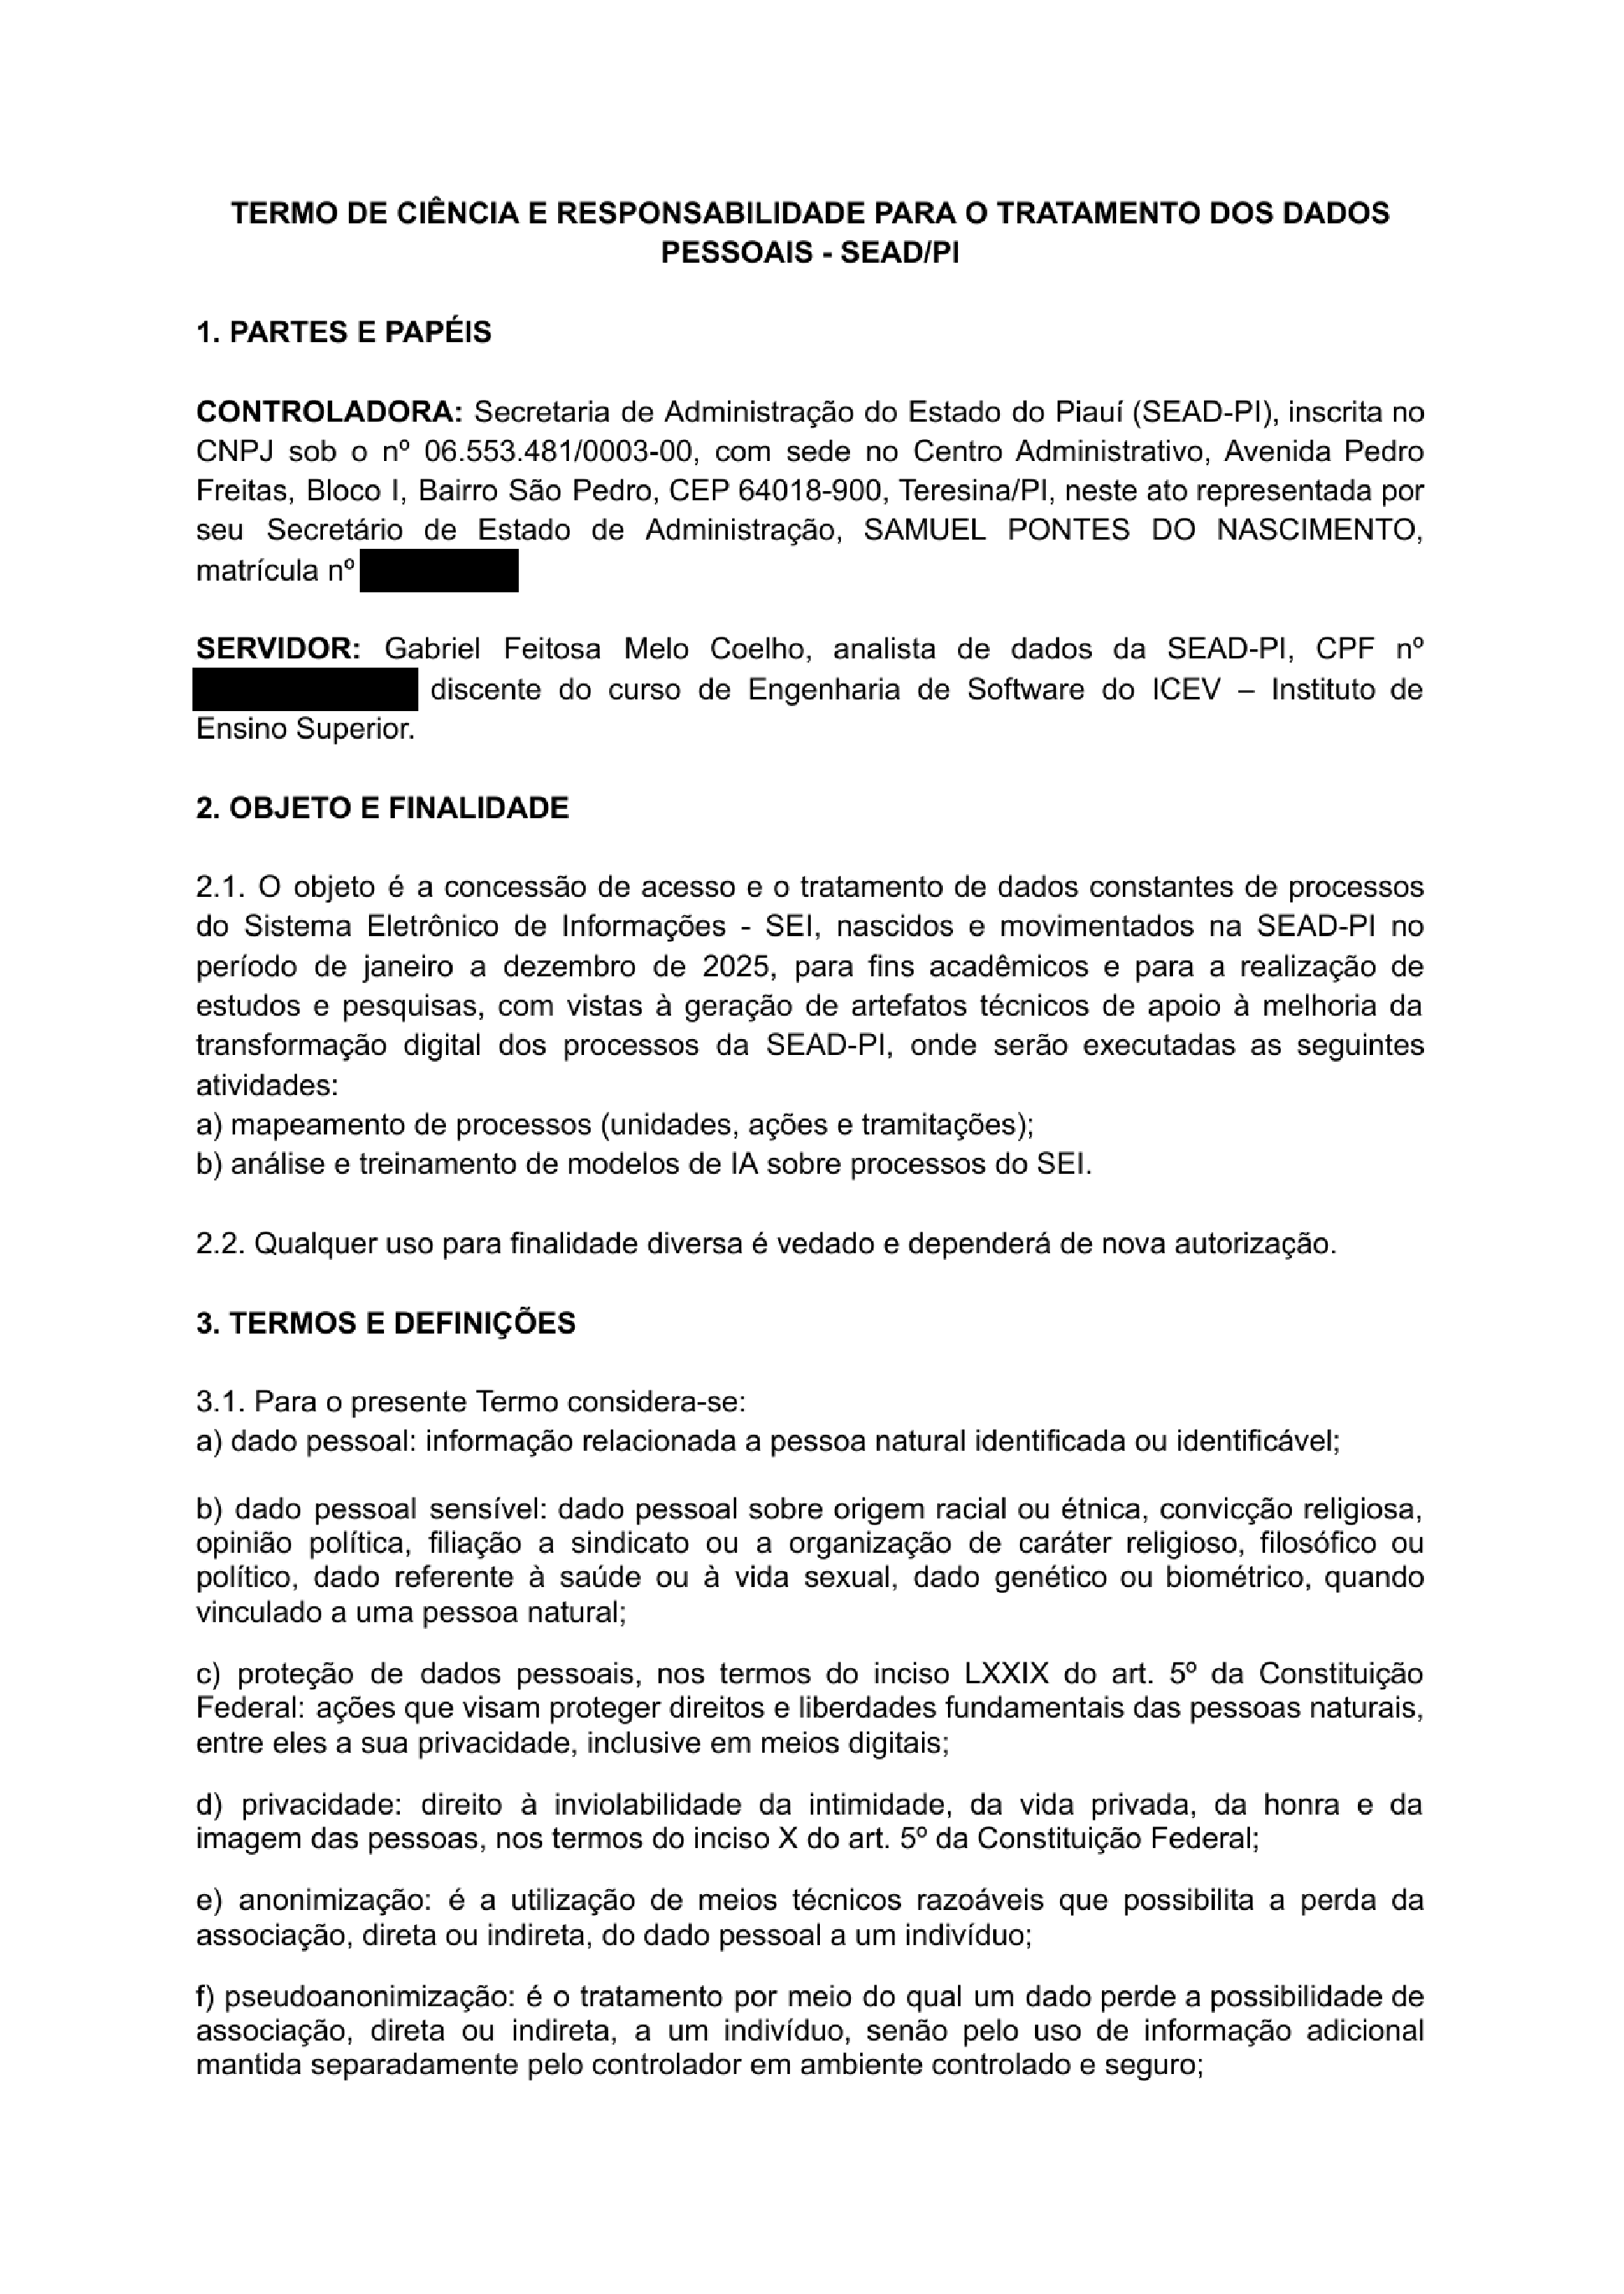
\includepdf[pages=-,frame,scale=0.88,pagecommand={}]{anexos/termo-autorizacao-tarjado.pdf}


\end{document}
